\documentclass{article}
\usepackage{allan}
\usepackage{lastpage}
\usepackage{algorithmic}
\usepackage{algorithm}
\usepackage{indentfirst}
%\RequirePackage{graphics}
% Replace ABCDEF in the next line with your chosen problem
% and replace 111111 with your Team Control Number
% and replace abcdef with your Title
% and replace 123456 with the number of pages of your essay
\setlength{\headheight}{70pt}
\newcommand{\Title}{Boarding and Disembarking a Plane}
\newcommand{\Team}{22768821}
\newcommand{\Problem}{}
\def\mathbi#1{\textbf{\em #1}}
%\newcommand{\itembf}{\item \textbf}
\title{\Huge\textbf{\Title}}
\author{Team\#\Team}
\date{\today}

\newcommand{\cA}{\color{allanblue}Constant A\color{black}}
\newcommand{\cB}{\color{allandarkblue}Constant B\color{black}}
\newcommand{\varr}{\color{allanpurple}Variable\color{black}}
%%%%%%%%%%%%%%%%%%%%%%%%%%%%%%%%%%%%%%%%
% set up of theorems

\newtheorem{thm}{Theorem}[section]
\newtheorem{cor}[thm]{Corollary}
\newtheorem{lem}[thm]{Lemma}
\newtheorem{prop}[thm]{Proposition}
\theoremstyle{definition}
\newtheorem{defn}[thm]{Definition}
\theoremstyle{remark}
\newtheorem{rem}[thm]{Remark}
\numberwithin{equation}{section}
\newtheorem{theorem}{Theorem}
\newtheorem{corollary}[theorem]{Corollary}
\newtheorem{lemma}[theorem]{Lemma}
\newtheorem{definition}{Definition}

%%%%%%%%%%%%%%%%%%%%%%%%%%%%%%%%%%%%%%%%
% setup of page length and script size

\setlength{\belowcaptionskip}{3.7pt}
\setlength{\abovecaptionskip}{4.7pt}
\setlength{\headsep}{0.35in}
\setlength{\headheight}{14.5pt}
\setlength{\parindent}{2em}
%\captionsetup{font={footnotesize}}
\renewcommand{\baselinestretch}{1}
%\setlength{\parskip}{0.28em}
\geometry{bottom=1in}



%%%%%%%%%%%%%%%%%%%%%%%%%%%%%%%%%%%%%%%%
%\lhead{
%   \parbox{5cm}{
%        \begin{center}
%            Problem Chosen \\[0.2cm]
%            \textbf{\Huge{A}}
%        \end{center}
%    }
%}
%\chead{
%    \parbox{5cm}{
%        \textbf{
 %           \begin{center}
%               2022 \\
%                MCM \\
%                Summary Sheet
%            \end{center}
%        }
%    }
%}
%\rhead{
%    \parbox{5cm}{
%        \begin{center}
%            Team Control Number \\[0.2cm]
%            \textbf{\Huge{2226594}}
%        \end{center}
%    }
%}
\cfoot{}
%IMMC Template
\chead{
    \parbox{5cm}{
        \textbf{
           \begin{center}
				Team Control Number\\[10pt]
				\textbf{\begin{Huge}\Team\end{Huge}}\\
				%Problem Chosen\\
				%\textbf{\Problem}\\
                2022 \\
                IMMC \\
                Summary Sheet
            \end{center}
        }
    }
}

\begin{document}
	\normalfont\fontfamily{qpl}\selectfont
    %\begin{center}
    %    \textbf{\large Summary}

    %\end{center}
	%%%%%%%%%%% Begin Summary %%%%%%%%%%%%%%%%%%
	% Enter your summary here replacing the (red) text
	% Replace the text from here ...
	\qquad
	\par
	~~
	\\


	%end Summary
	%%%%%%%%%%%%%%%%%%%%%%%%%%%%%%%%%%%%%%%%%%%%%%%%%%%%%%%%%%%%%%%%
	% real document begins
    %%%%%%%%%%%%%%%%%%%%%%%%%%%%%%%%%%%%%%%%%%%%%%%%%%%%%%%%%%%%%%%%
	\clearpage
    \pagenumbering{arabic}
    \newpage
    \pagestyle{empty}
    \setlength{\headheight}{12pt}
    \renewcommand{\headrulewidth}{0.5pt}
    % \renewcommand{\headrulewidth}{5cm}
    \renewcommand{\footrulewidth}{0.0pt}
    \pagestyle{fancy}
    \lhead{Team \#\Team}
    \chead{\Title}
    \rhead{Page \thepage\ of \pageref{LastPage}}
    \cfoot{}
    \lfoot{}
    \rfoot{}

    %%%%%%%%%%%%%%%%%%%%%%%%%%%%%%%%%%%%%%%%%%%%%%%%%%%%%%%%%%%%%%%%
    \clearpage
    \thispagestyle{empty}
    \tableofcontents
    \newpage
    \pagestyle{fancy}
    \setcounter{page}{1}

	\newpage
	\section{Introduction}
	\subsection{Background}
	Time and efficiency play a vital role in air transportation. During normal passenger flights, sections which require a great smount of time include \defword{boarding} and \defword{disembarking} of passengers. Therefore, it's necessary to build a model which provides the best strategy for different plane types and on various occasions.

	There are a variety of boarding and disembarking methods used by air companies now. In one plan, passengers appear in the plane with no plans devised in advance. In other strategies, passengers enter the plane according to their row numbers, seat positions or priority (E.g. first class \& economic class), etc. However, not all of the passengers obey the rules, so there emergency events occur from time to time.

	While boarding a plane, passengers will first go to their assigned seat, put their luggage on the rack and then get seated. While a passenger stowing their bags, other travellers who are stuck behind in the queue and haven't reached their target seats should wait until the passenger finishes the process, resulting in a queue. The image below descibes the process in which the passengers placing the bags cause a queue.


	\begin{center}
		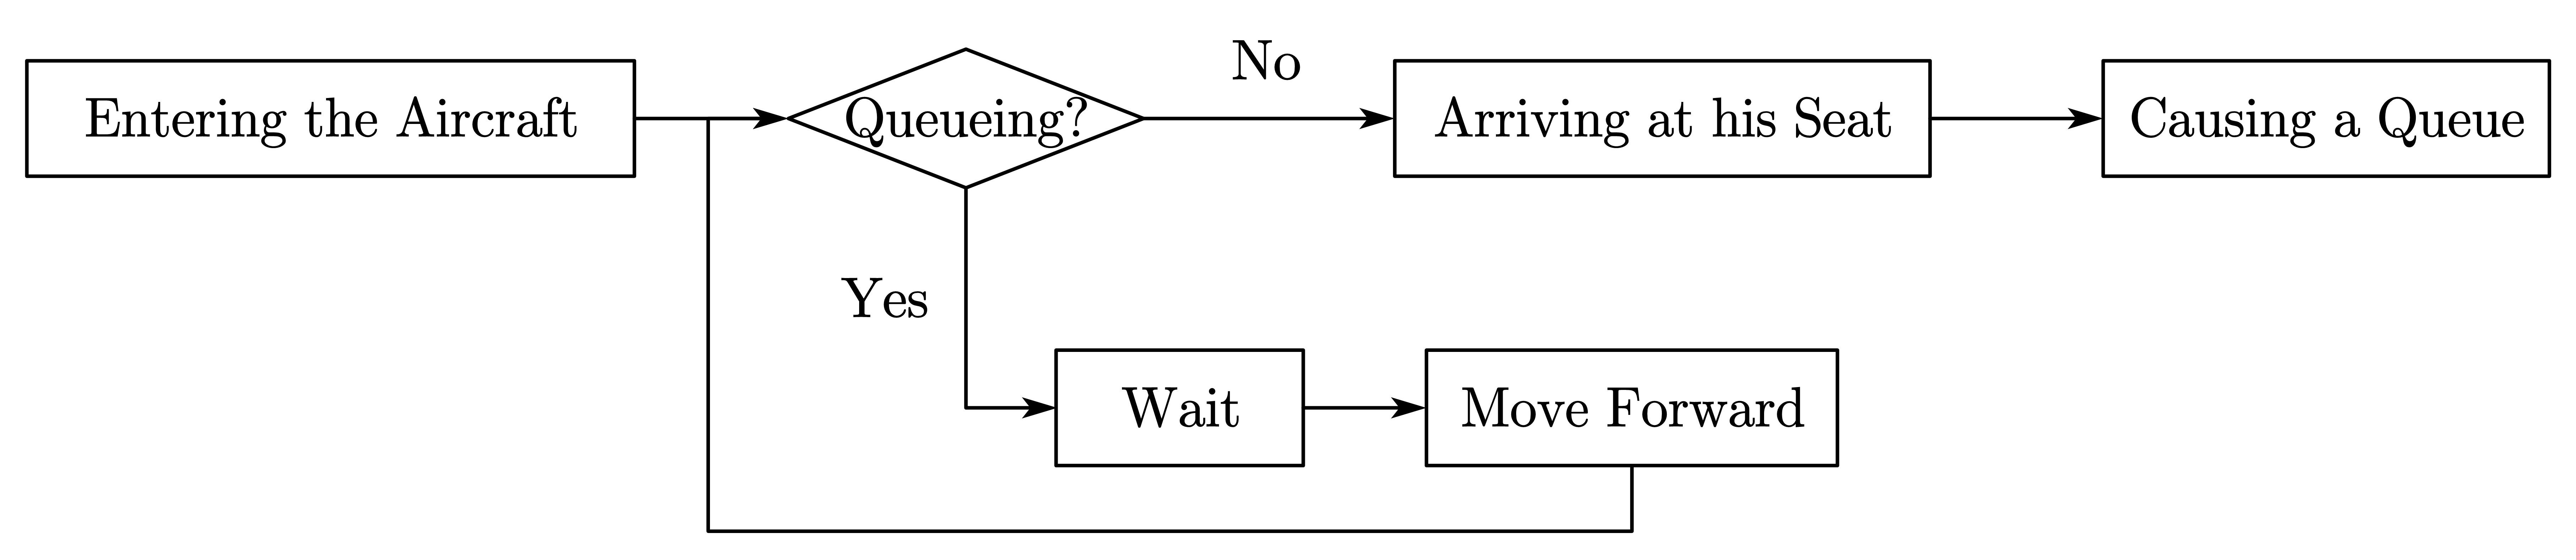
\includegraphics[width=14cm]{chart.jpg}

		\textit{Fig. 1 Boarding process of a specific passenger}
	\end{center}

	Moreover, it's important to note that if other seats have been occupied, its necessary for some passengers to stand up in order to provide unseated passengers with more space to reach their seat.

	In contradiction to the boarding process, the main problem of the disembarking process is that passengers who are eager to get out the plane may block the plane while they are taking their carry-on bags. This requires careful planning so that they will not stop the passengers on the back rows from moving.
	\subsection{Our Work}
	In our model, we need to find out the best strategy which suits the plane type perfectly. Therefore, our work is divided into 3 parts.
	\begin{itemize}
		\item Design a model which can calculate the time required to board and disembark when applied to all kinds of planes.
		\item Improve the model considering different situations and emergency events and design a brief strategy based on the results of our model.
		\item Apply our model to real-life planes and find out the best strategy which minimizes the boarding and disembarking time.
	\end{itemize}
	\subsection{General Assumptions}
	\begin{enumerate}
		\itembf{For each passenger, their luggage is put on the rack above them.}

		Airlines usually ensure this fact to minimize unnecessary congestion
		\itembf{For a certain passenger, the time to lay down his luggage and the time to remove it is the same.}

		This process can be mathematically acknowledged as \defword{reversible} (Consider when time relapses).
		\itembf{The total width of a passenger and his luggage is similar to the width between rows.}

		To provide the passengers the best flying experience, the flying company need to find a width between rows which will both satisfy the needs of people and maximize the plane's capacity.
		\itembf{All passengers walk in the same speed on the aisles.}

		Though there are energy difference caused by age and sex, there is slight difference of walking velocity when different passengers walk on a plane searching for their assigned seat. Therefore, we can neglect the difference and assume that all the passengers have the same ideal velocity.
		\itembf{Passengers never go backward.}

		Most passengers concentrated on finding their seat most. Therefore, they seldom miss their way and try to move backward.
		\itembf{First and business class passengers are prioritized with respect to those of the economic class.}

		Although (according to the ultimate results displayed in our essay), this is not the best boarding strategy for any types of plane and passengers, letting distinguished guests board first will give these passengers a sense of \defword{satisfaction} and enlarge the airline company's income. Therefore, we took this fact into consideration to make our model more realistic.
	\end{enumerate}
	\section{Model A: Finding the fastest strategy}
	\subsection{Model Overview}
	In this part, we will assess the plane and get the formulae desribing time sonsumption in boarding and disembarking. We define each seat as a block which has their own properties. All of the blocks belong to a coordinate divided accroding to the plane's overall arrangement. Later, we will get out the spent to move to these blocks also based on different moving conditions.
	\subsection{Assumptions}
	\begin{enumerate}
		\itembf{The luggage racks are designed to be adequate for any reasonable amount of luggage.}

		Consignment service is provided with the passengers before they enter the plane. Therefore, we can assume that there are enough space for the passengers to place smaller items, which means the space for storage is endless.
		\itembf{In a certain cell, $v$ is a fixed value.}

		Since $d$ (the width between rows, or the length of a cell) is taken as 0.8$\mathrm{m}$, a very small distance, there won't be a big difference in velocity change when a passenger is moving in the cell. Therefore, we can assume that $v$ in a certain block won't change.
	\end{enumerate}
	\subsection{Notice}
	In our model, we set \(\tau_0=1\mathrm{s}\) as the basic simulation unit, meaning that the model is also distrete. In an effort to standardize time and distance discretely, we make the following definitions in the rest of the model, (both \textit{time} and \textit{velocity} have no dimensions):
	\begin{itemize}
		\item \textbf{time}:
			For a period of \(t\,\mathrm{s}\) in \textit{SI}, we define the actual simulation time as \(t'=\dfrac{t}{\tau_0}\), which literally represents how many \(\tau_0\) s \(t\) consists of.
		\item \textbf{speed}:
			While a speed measuring \(v\,\mathrm{m\cdot s^{-1}}\) in reality means that the object travels \(v\,\mathrm{m}\) in a second, we define \defword{velocity} \(v'\) as the amount of \defword{time} (the \textit{time} here refers to the one as defined above) that takes the object to move \(d\), i.e. the length of a \textit{cell}. Therefore we have the following relationship between the two types of speeds:\[v=\dfrac{d}{v'\cdot \tau_0}\,\left(\mathrm{m\cdot s^{-1}}\right)\]
	\end{itemize}
	\subsection{Notations}
	We classify \textit{notations} into the following three types:
	\begin{itemize}
		\item \cA: won't change in the whole scope.
		\item \cB: may change in the whole scope, but won't change for a fixed set of passengers and a set plane.
		\item \varr: varies for different initial sequences of passengers.
	\end{itemize}
	\begin{center}
	\begin{tabular}{|l|l|l|l|}
		\hline
		$\tau_0$&simulation interval taken in our model, about \(1 \,\mathrm{s}\)&$\mathrm{s}$&\cA\\
		\hline
		\(\tau\)&simulation time step\(=\frac{\tau_0}{6}\)&\(\mathrm{s}\)&\cA\\
		\hline
		\(D\)&number of cells in the observable area, taken as \(4\,\left(\mathrm{persons}\right)\)&1&\cA\\
		\hline
		\(t\)&current time&1&\varr\\
		\hline
		$d$&width of each cell&$\mathrm{m}$&\cA\\
		\hline
		$N$&total number of passengers on the plane&1&\cB\\
		\hline
		$v_0$&maximum walking speed of a passenger aboard&1&\cA\\
		\hline
		$t_L (A)$&standard time for a passenger $A$ to place his luggage&1&\cA\\
		\hline
		$t_s$&time for a passenger to horizontally move a seat's length&1&\cA\\
		\hline
		$P$&the set of all passengers&/&\cB\\
		\hline
		$M$&number of cells on aisles&1&\cB\\
		\hline
		$C\left( A,t \right)$&the cell passenger $A$ is located at time $t$&1&\varr\\
		\hline
		$P_v\left( A \right)$&number of passengers visible within $D$ blocks before him&1&\varr\\
		\hline
		$S_i\left( A \right)$&total time needed to pass the first $i$ cells& 1&\varr\\
		\hline
		$v_i\left( A \right)$&the speed of passenger $A$ in the \(i^{\mathrm{th}}\) cell&1&\varr\\
		\hline
		$\tau _i\left( A \right)$&the time passenger $A$ spent in the $i^\text{th}$ cell&1&\varr\\
		\hline
		$v\left( A,t \right)$&the speed of passenger $A$ at $t$&1&\varr\\
		\hline
		$\gamma \left( A \right)$&non-compliance index of \(A\)&1&\cB\\
		\hline
		$l_i\left( A \right)$&whether the passenger $A$ is placing his luggage \(\in\left\{0,1\right\}\)&1&\varr\\
		\hline
		$\varepsilon \left( A \right)$&the time passenger $A$ need to be offered the seat&1&\varr\\
		\hline
		$\psi \left( A \right)$&time passenger $A$ to seat after starting putting luggage&1&\varr\\
		\hline
		$T\left( A \right)$&total boarding time of passenger $A$&1&\varr\\
		\hline
		$\Gamma$ &total boarding time&1&\varr\\
		\hline
		\(r\)& parallelity index& 1& \varr\\
		\hline
	\end{tabular}
	\end{center}
	\subsection{Moving State of Passenger $A$}
	In this part, we mainly focus on how to describe the passengers. We saperate the plane into different \defword{cells}. Each cell has several properties describing its location, type (such as seats and aisles) and other properties. In special kinds of planes where the seats are arranged in irregular graphics, we still add them to the matrix, but we will not put them into consideration when it comes to calculations.

	First we will discuss the passenger's miving condition. To better describe the state of the seats, we define a simulating time step $\tau$, which equals $\dfrac{\tau_0}{6}$ ($\frac{1}{6}\mathrm{s}$). Under ideal circumstances, a passenger will move at a constant speed $v_0$. In our model, the smaller $v_0$ is, the faster the passenger travels.

	\begin{center}
		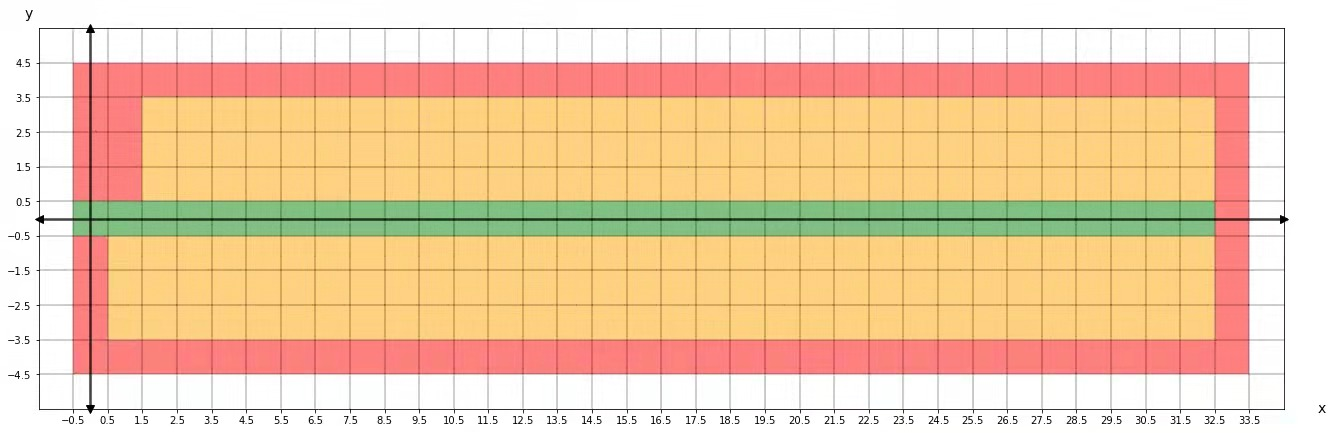
\includegraphics[width = 14cm]{cell_visualization.jpg}

		\small\textit{Fig. Construction of cells}
	\end{center}

	The following process will give the relationship solely between \(v\) in the aspect of both space and time.
	\subsubsection{Step One: \(v\to P_v\)}
	First, it's obvious that the more jammed a person is, the slower he or she moves. Therefore, it's important to first define \defword{density}.

	We define \defword{density} as the ratio of the number of people in the visible area to the number of cells in that visibility region. On an airplane, we take \textit{the number of cells in a passenger's visibility region} as \(4\), meaning that cells farther than that have no effects on the passenger. We have:
	\[\mathrm{Density\left(A\right)} = \dfrac{P_v\left(A\right)}{D}\]

	And according to the widely-adopted Greenshields speed-density linear model (\Huge CITE.\normalsize), \[\mathrm{congested\:speed} = \mathrm{normal\:speed}\cdot\left(1-\mathrm{Density\left(A\right)}\right)\]

	By converting the physical \textit{velocity} into our unit, we have the following equation by definition:
	\[v(A)=\begin{cases}\dfrac{v_0}{1-\mathrm{Density\left(A\right)}}=\dfrac{v_0}{1-\frac{P_v\left(A\right)}{D}}, \text{if the passenger ahead is walking}\\\infty, \text{the passenger ahead stops}\end{cases}\]
d
	When \(v\left(A\right)=\infty\), the traditional way of calculation can no longer be used to calculate displacement. Therefore, we suppose that the passenger enters a state where he can't move until the person causing the queue gets seated. Currently we adopt the searching method to record that specific person, but later we will introduce a new concept \textit{cluster} to solve this problem.
	 After calculations, we've got the relationship between velocity and density.
	\subsubsection{Step Two: \(P_v\to \) passenger distribution}
	There clearly is a pretty logical way of ergodicing all the positions each time and get the respective \(P_v\left(A\right)\) for every passenger. But in order to achieve this with pure mathematics, we introduce the \textit{existence} factor and the \textit{effective} factor, both of which are included in the vector. Only when these two both have an effect on the passenger \(A\) can the index \(P_v\left(A\right)\) be taken into consideration.

	The first vector in the multiplication is the \textit{effective} factor, meaning that only people within the visibility range of \(A\) have an effect on him/her.

	\begin{center}
	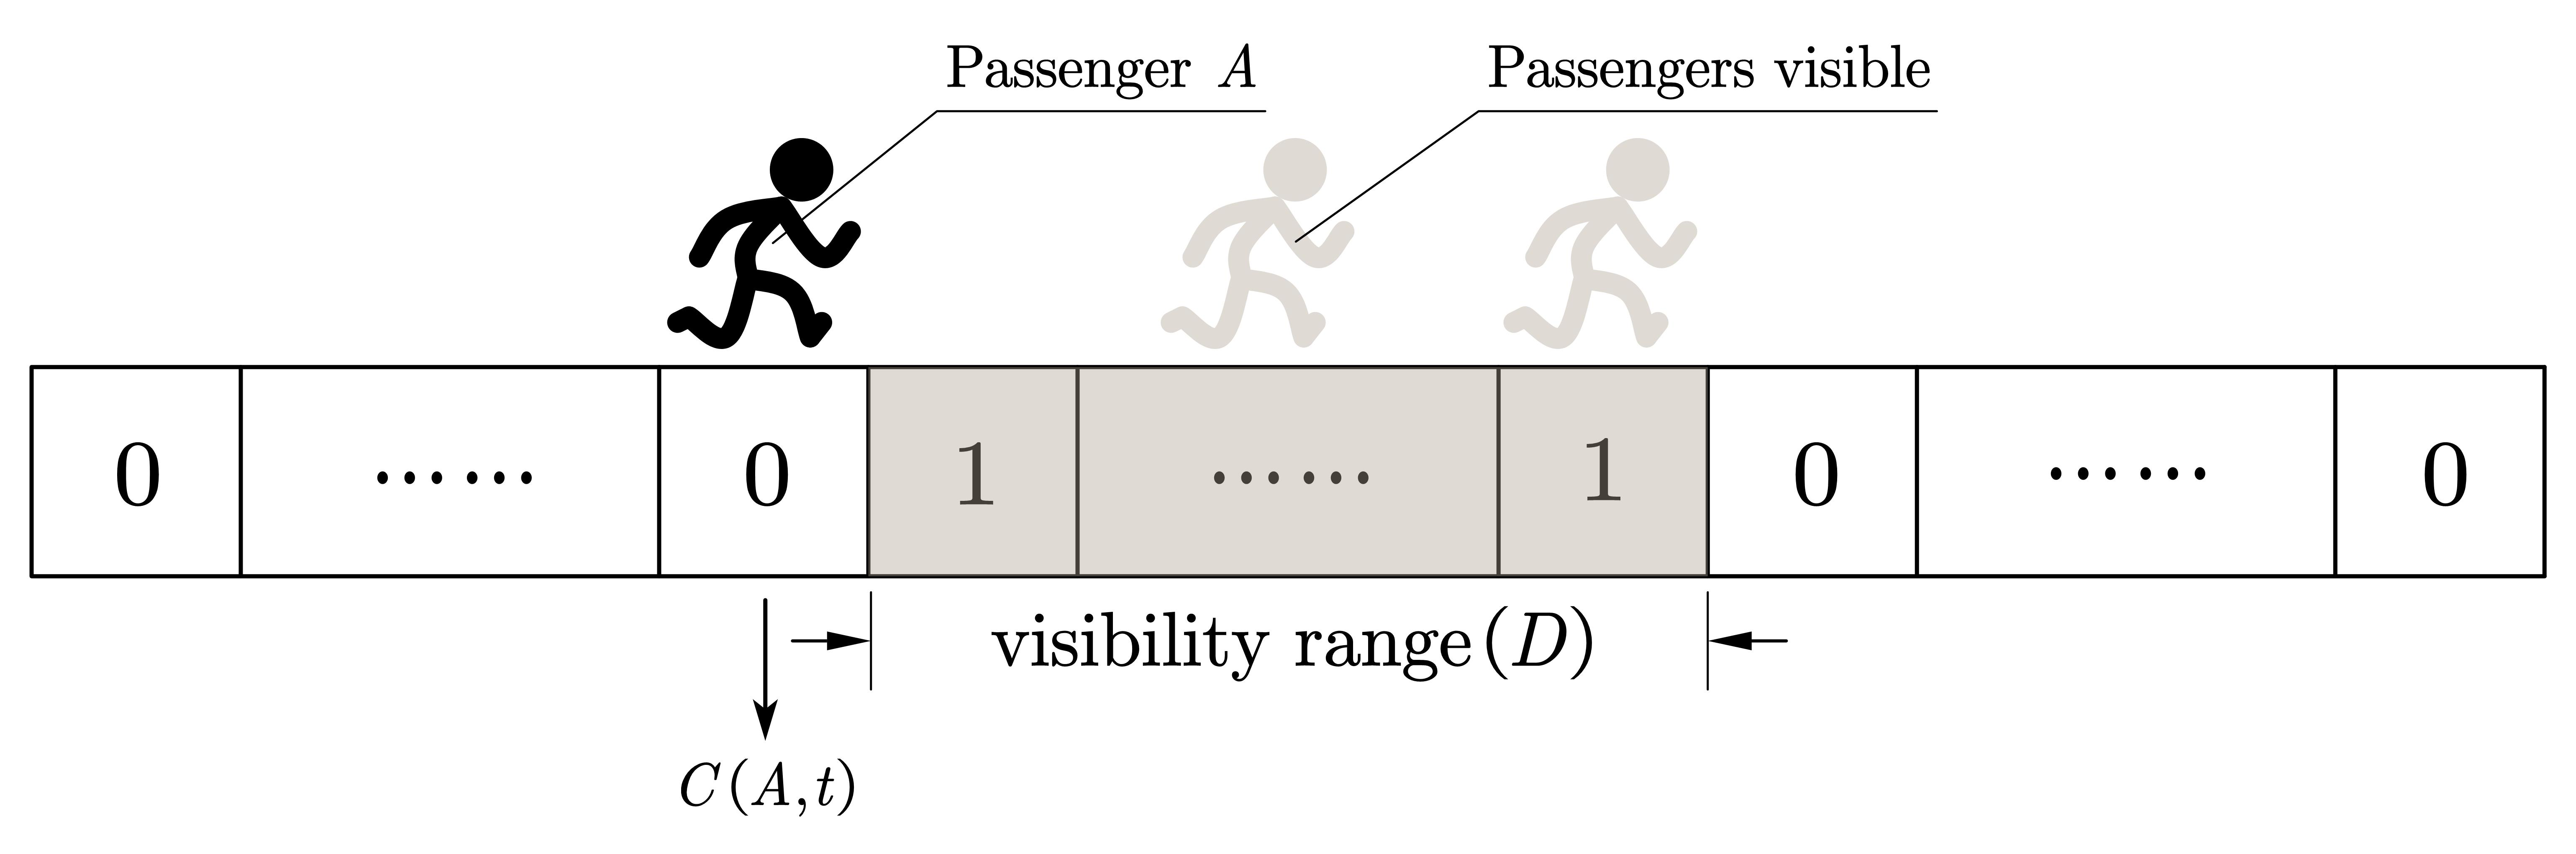
\includegraphics[width = 11cm]{effective factor.jpg}

	\small\textit{Fig. The effective factor}
	\end{center}

	The second vector is the \textit{existance} factor, indicating whether there exists anyone in each cell, which is also the \(0-1\) distribution for the whole group of cells. It can also be calculated by simply adding all the positions together.
	\[\text{Existance factor} = \text{Distribution of positions} = \sum\limits_{A\in P} \text{the position of }A\]

	By multiplying these two, we get the formula of \(P_v\left( A \right)\):

	$$P_v\left( A \right) =\left( 0,...0,\underset{D\:\mathrm{amount}\:\mathrm{of}\:1\mathrm{s}}{\underbrace{1,...,1}},0,...,0 \right) \times \left[ \sum_{A\in P}{\left( 0,...,0,\underset{\mathrm{the}\:C\left( A,t \right) ^{\mathrm{th}}\,\,\mathrm{position}\:\mathrm{from}\:\mathrm{top}\:\mathrm{to}\:\mathrm{bottom}}{\underbrace{1}},0,...,0 \right) ^{\top}} \right] $$
	\subsubsection{Step Three: passenger distribution \(\to \) individual \(v\)}
	According to our assumptions, it's easy to find that every passenger will move more slowly than the passenger ahead of him. Therefore, each initial sequence yields a distinctive position set.

	We define \(S_i\left( A \right)\) as the time used to cover the distance of \(i\) cells:
	$$S_i\left( A \right) \xlongequal{\mathrm{def}}\sum_{j=1}^i{v_j\left( A \right)}>0$$

	With the formula above, it's easy to determine the current cell of \(A\):
	$$C\left( A,t \right) =\min_{\substack{\frac{t}{S_i\left( A \right)}\le 1\\1\le i\le M\\}} \left\{ i \right\} $$
	(In this model, $C(A,t)$ can be considered as a linear combination of $v$.)
	\subsubsection{Final Step: \(v\to v\)}
	Summing up the previous three parts, we can identify $v(A,t)$, which is demonstrated in the following formulae:
	$$v\left( A_l,t \right) =\frac{v_0}{E_l+\sum\limits_{\alpha =1}^N{\left( \sum\limits_{\beta =1}^T{\left( \lambda _{\alpha ,\beta}^{\left( l \right)}\cdot v\left( A_{\alpha},\beta \right) \right)} \right)}}\left( l\in \left\{ 1,2,...,N \right\} ,E_l\in \mathbb{R} \right)$$
	where
	$$\sum_{\alpha =1}^N{\left( \sum_{\beta =1}^T{\left( \lambda _{\alpha ,\beta}^{\left( l \right)}\cdot v\left( A_{\alpha},\beta \right) \right)} \right)}=\frac{v_0}{v\left( A_l,t \right)}-E_l\left( l\in \left\{ 1,2,...,N \right\} ,E_l\in \mathbb{R} \right)$$
	is a linear combination of the velocities. (Notice that not only process three but also the first two steps ensure linearity)
	\subsubsection{Putting luggage and Offering seats}
	Next we calculate the time spent while one is trying to take his/her seat.
	\begin{itemize}
		\item \defword{\textbf{Stowing luggage.}}

		The standard stowing time has already been given as \(t_L\). However, the time does not always remain unvariant. Due to the fact that different passengers bring different amounts of luggage aboard and that some passengers disobey boarding rules, we introduce a non-compliance index \(\gamma\left(A\right)\). The higher \(\gamma\left(A\right)\) is, the more time it takes \(A\) to stow his/her luggage.

		Therefore, the overall time \(A\) consumed to stow his/her luggage equals:
		\[\text{stowing time}=\gamma \left( A \right) t_L \]
		\item \defword{\textbf{Getting seated.}}

		In some strategies, passengers near the aisle have to stand up to let a new traveller get through. (In other strategies such as \textit{window middle aisle}, this scenario never occurs). We add a special property to each cell which determines whether the cell is being seated. When the passenger outside has been seated and the other two passengers inside come, the passenger needn't stand up twice to offer his seat. Therefore, we can describe the time spent in seating as:
		$$t(1,k)=v_0$$
		$$t(A,a)=\begin{cases}t(A-1,a+1),\text{there is a person on the $a+1$ block}\\v_0, \text{the \textbf{a+1} block is empty}\end{cases}$$

		To form equations, we adopt motional physics and according to our assumptions, the time consumed to offer seat is proportional to the distance one moves, which is then proportional to the number of seats separating one from the aisle.
		\begin{center}
		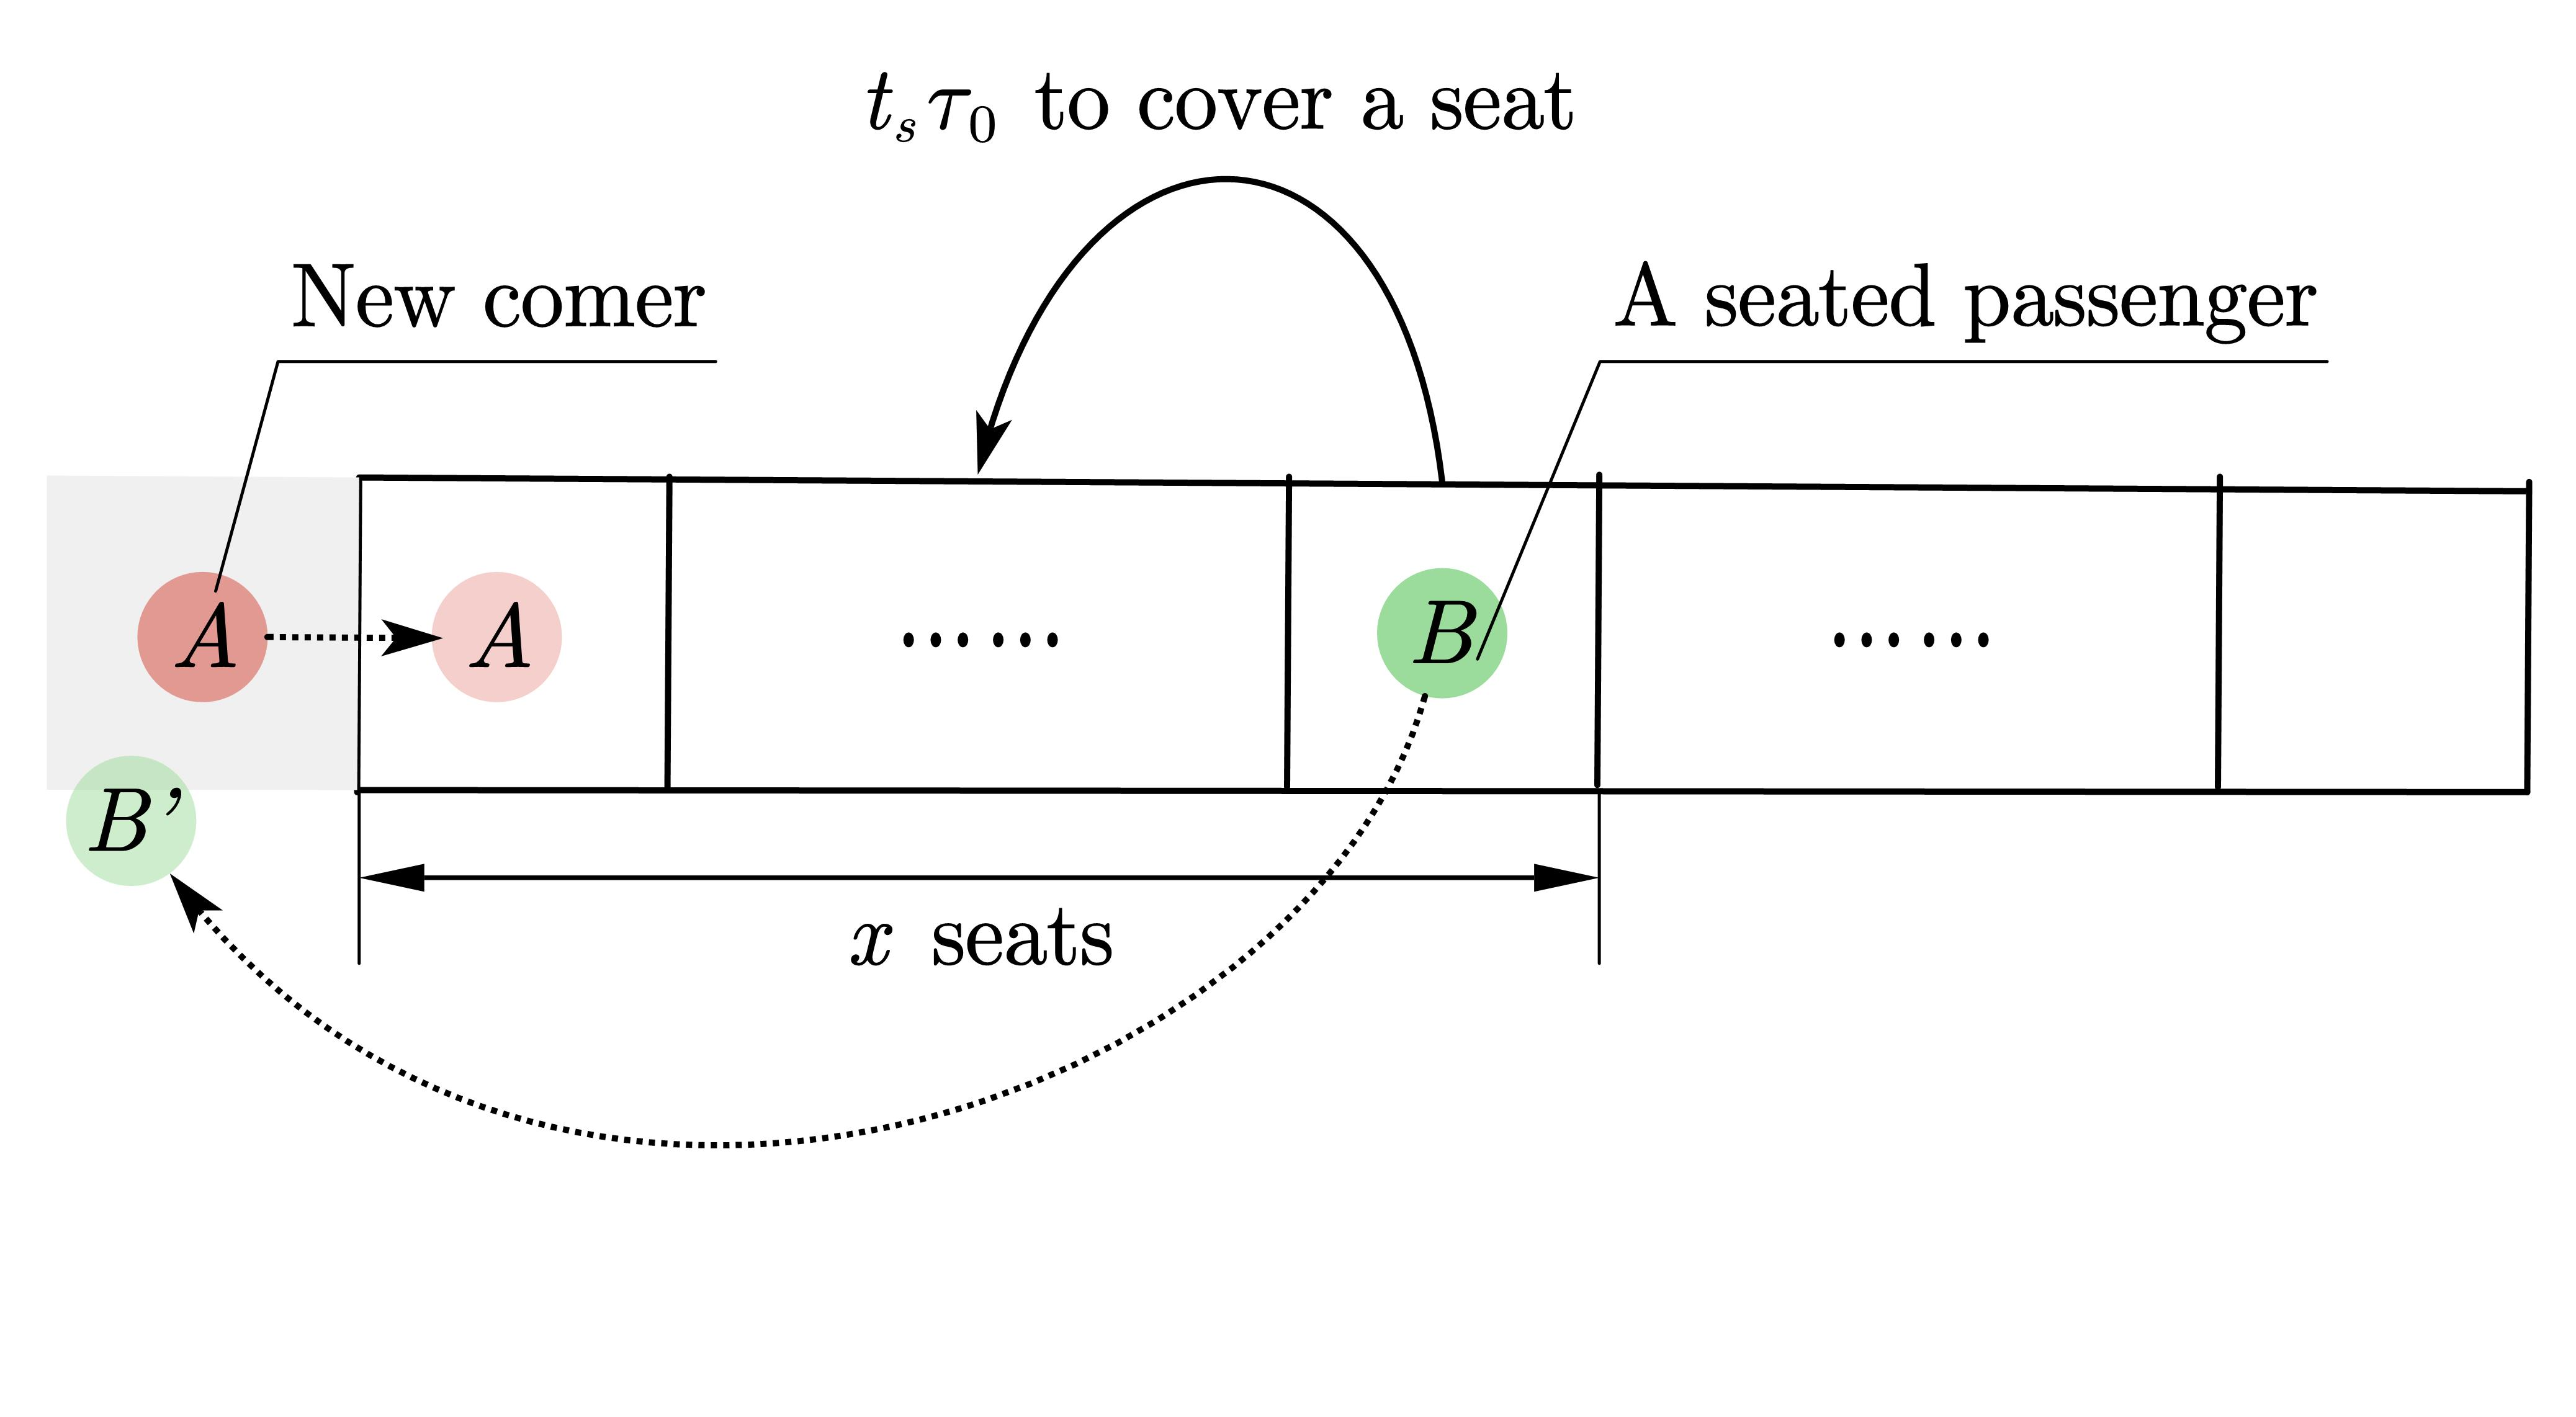
\includegraphics[width = 10cm]{offering a seat.jpg}

		\small\textit{Fig. Offering a seat}
		\end{center}

		So when he/she travels $x$ cells, the total time \(B\) consumed equals:
		$$t(B)=x\cdot t_s \cdot \tau_0$$

		And we take the maximum of the time to offer seats in this line as the total:
		\[\text{time to offer seat}=\max\limits_{B\in \text{this line}}\left\{t(B)\right\} = \max\limits_{B\in \text{this line}}\left\{x_{B}\cdot t_s \cdot \tau_0\right\}\]

		Once the passenger takes his/her seat, the cell on the aisle is no longer occupied, which ends the queueing process.
	\end{itemize}
	We introduce a special variable $l_i(A)$ to describe the passengers state. If he stops to place his luggage, \(l_i(A)=1\). Conversely, \(l_i(A)=0\). Below is given the two types of states of passenger \(A\):
	\[\Xi_i\left(A\right)=\left( \begin{matrix}
	l_i\left( A \right)&		\\
	&		1-l_i\left( A \right)\\
	\end{matrix} \right) \in \mathbb{R}^2\cap \left\{ \left( \begin{matrix}
	0&		\\
	&		1\\
	\end{matrix} \right) ,\left( \begin{matrix}
	1&		\\
	&		0\\
	\end{matrix} \right) \right\}\]

	In additon, we define $\psi(A)$ to descibe the total time passenger $A$ spent from stopping placing his luggage to sitting down. It is clear that $\psi \left( A \right) =\max \left\{ \epsilon \left( A \right) ,\gamma \left( A \right) t_L \right\}$.

	\subsubsection{Calculating total time}
	Next, we calculate the total time a passenger spends in cell \(i\) with the previous parts combined. This can be done through adding those together. Therefore, we can define the time passenger $A$ spent in the $i^\text{th}$ cell as:
	$$\tau _i\left( A \right) =v_i\left( A \right) +l_i\left( A \right) \cdot \psi \left( A \right) +\underset{\mathrm{whether}\:\:\mathrm{he}/\mathrm{she}\:\:\mathrm{needs}\:\:\mathrm{to}\:\:\mathrm{queue}}{\underbrace{\left( 1-l_i\left( A \right) \right) }}\cdot \psi \left( \mathrm{queuing}\:\:\mathrm{origin} \right)$$
	or in other words:
	\[\Xi _{\mathrm{full}\:\mathrm{state}}=\left( \begin{matrix}
	v_i\left( A \right)&		\\
	&		\Xi _i\left( A \right)\\
	\end{matrix} \right) \times \left( \begin{matrix}
	\text{whether moving}&		&		\\
	&		\text{whether stowing}&		\\
	&		&		\text{whether waiting}\\
	\end{matrix} \right) \]

	Finally, we can get the total time $A$ spent in boarding $T(A)$:
	$$T\left( A \right) =\sum_{i=1}^M{\tau _i\left( A \right)}$$
	(If $i$ is beyond \(A\)'s target, $\tau_i(A)=0$)

	And by calculating the total boarding time of each passenger and put them in order, we can find out:
	$$\Gamma =\max_{1\le i\le N} \left\{ T\left( A_i \right) \right\}$$
	\subsection{Optimization}
	In this part, we'll use various mathematical methods to give the fastest possible boarding strategy.
	\subsubsection{Parallel boarding}
	We noticed that the passengers in the rows in the left and those in the rows in the left wouldn't disrupt each other, for they do not share much space of the aisles. So a good strategy is to board some passengers in the left and some in the right at the same time. However, if we arrange the order strictly from the two sides to the middle, there would be too much queueing in the middle rows.

	To reduce the queueing, we can first divide the aircraft into eight groups of seats, each of which contains three rows. Then, we can board passengers in group $n$ and group $n+4$ together. This would not cause much queueing, and can also maximize efficiency by \defword{parallel boarding}.

	We define the \defword{parallelity index} \(r\) as the portion of cells that are in the stowing state to the number of total aisle cells inside the plane: (In the first example, for instance, this total number equals \(33\).)
	\[r\left(t\right) = \dfrac{\#\text{cells in stowing state}}{\#\text{cells inside the plane}}\ddef\dfrac{C_s}{C_p}\]

	In intuition, the fastest strategy comes when everyone is blocked by one queuing origin each time, meaning that there may be \(C_s=C_p\) passengers stowing luggage but only costs a total of \(1\times t_L+o\left(1\right)\) amount of time, where \(o(1)\) is a constant relyin only on the passenger set and the plane type, which can greatly help reduce total time. To prove this, we use the attributes of discrete optimizations and get the aids by the computer.
	\begin{center}
		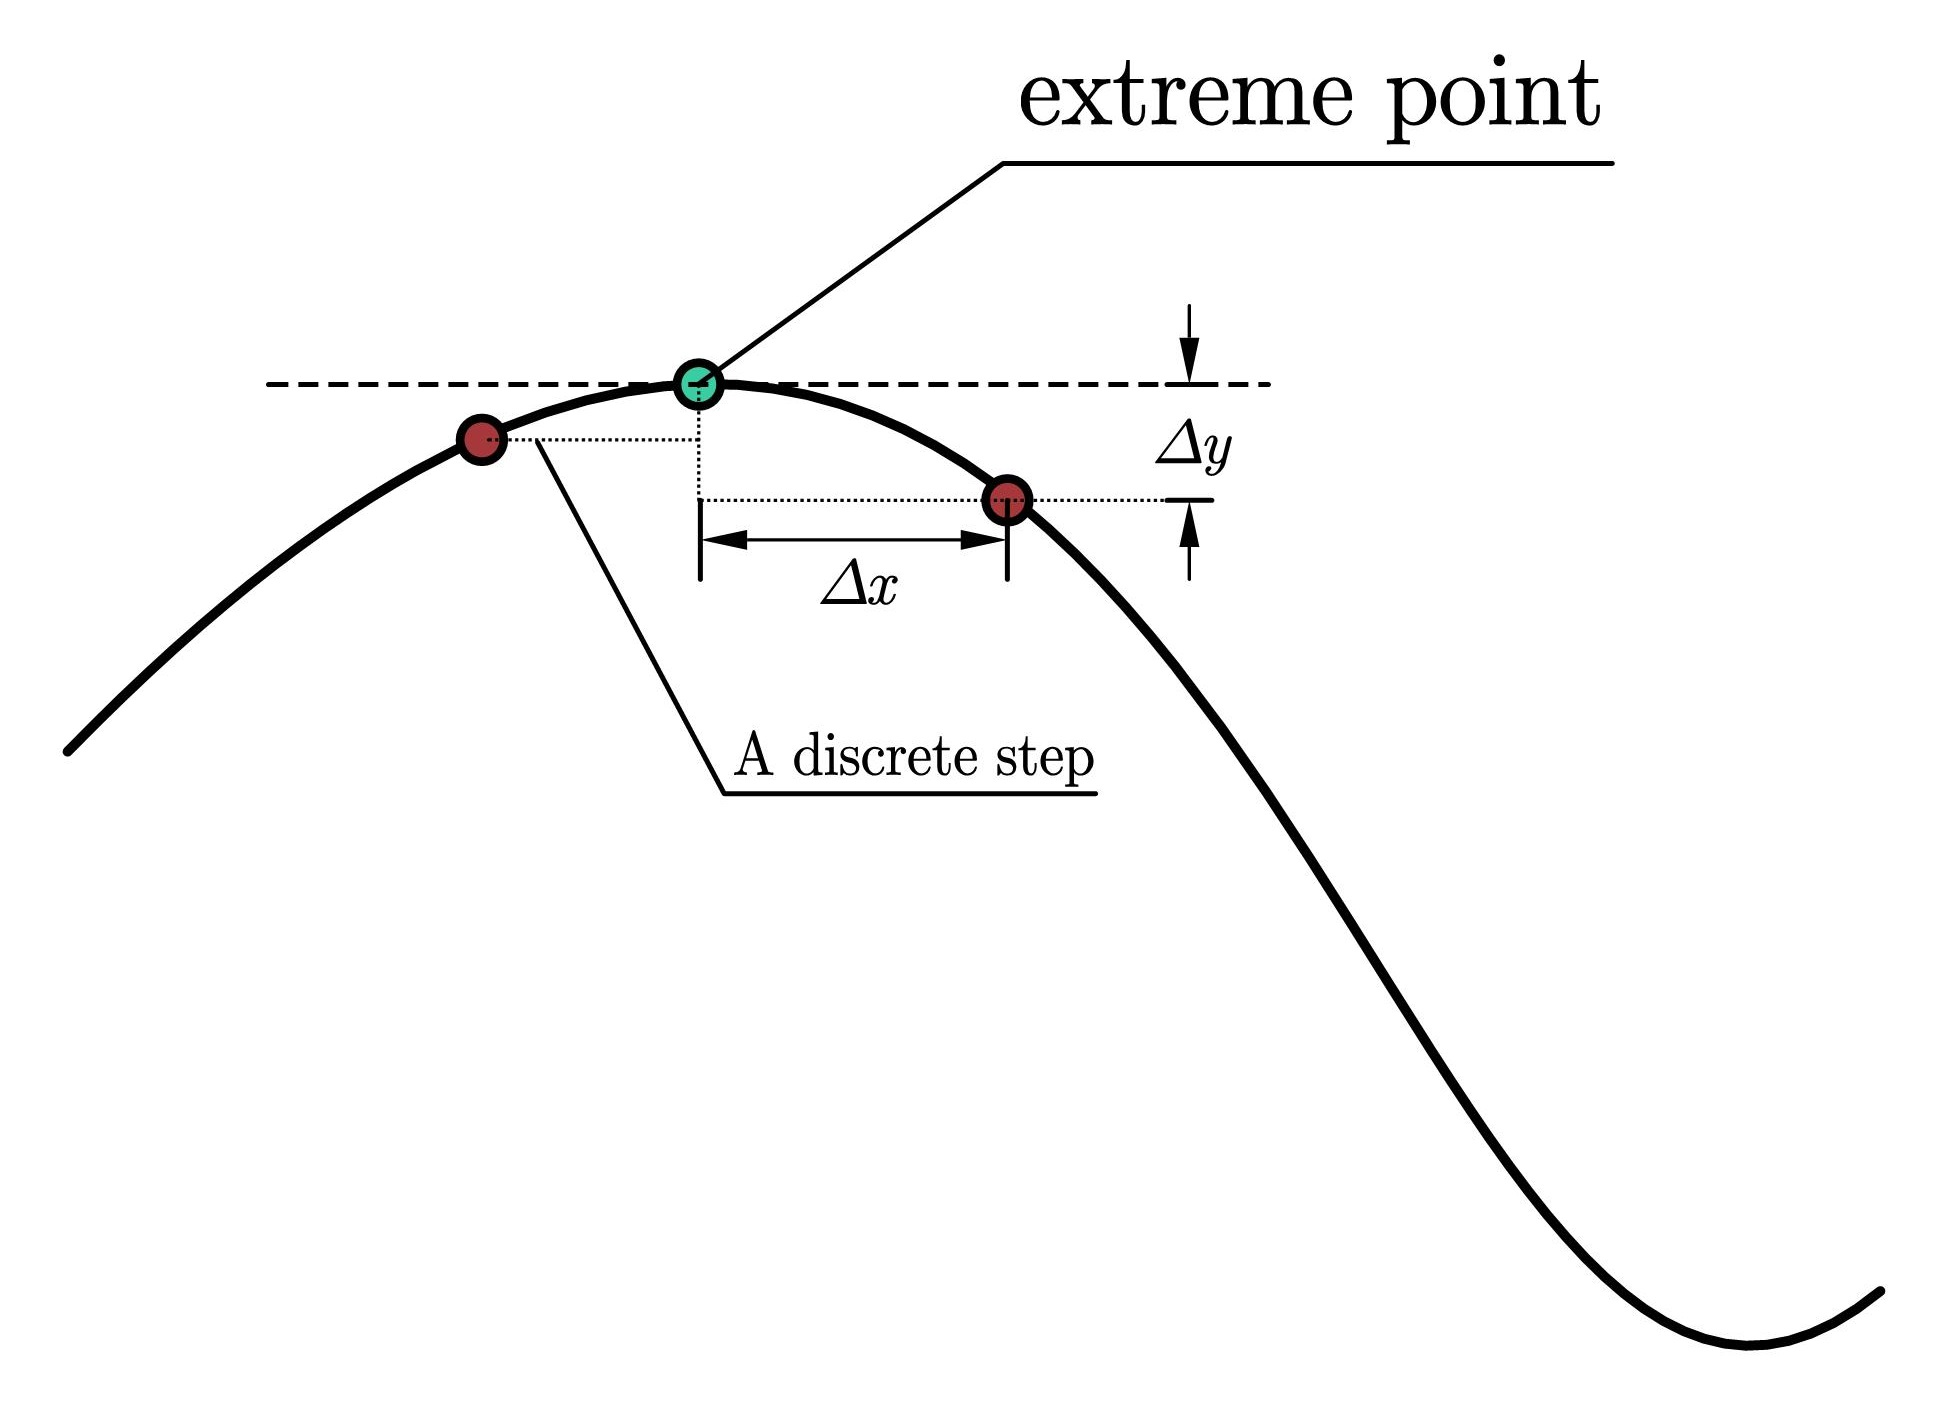
\includegraphics[height = 5cm]{discrete optimization.jpg}

		\small\textit{Fig. Discrete optimization}
	\end{center}

	\subsubsection{Computer-aided optimization}
	After adopting the discrete optimization model and with the \defword{parallelity} nature, we get the following ideal boarding plans:

	\begin{center}
		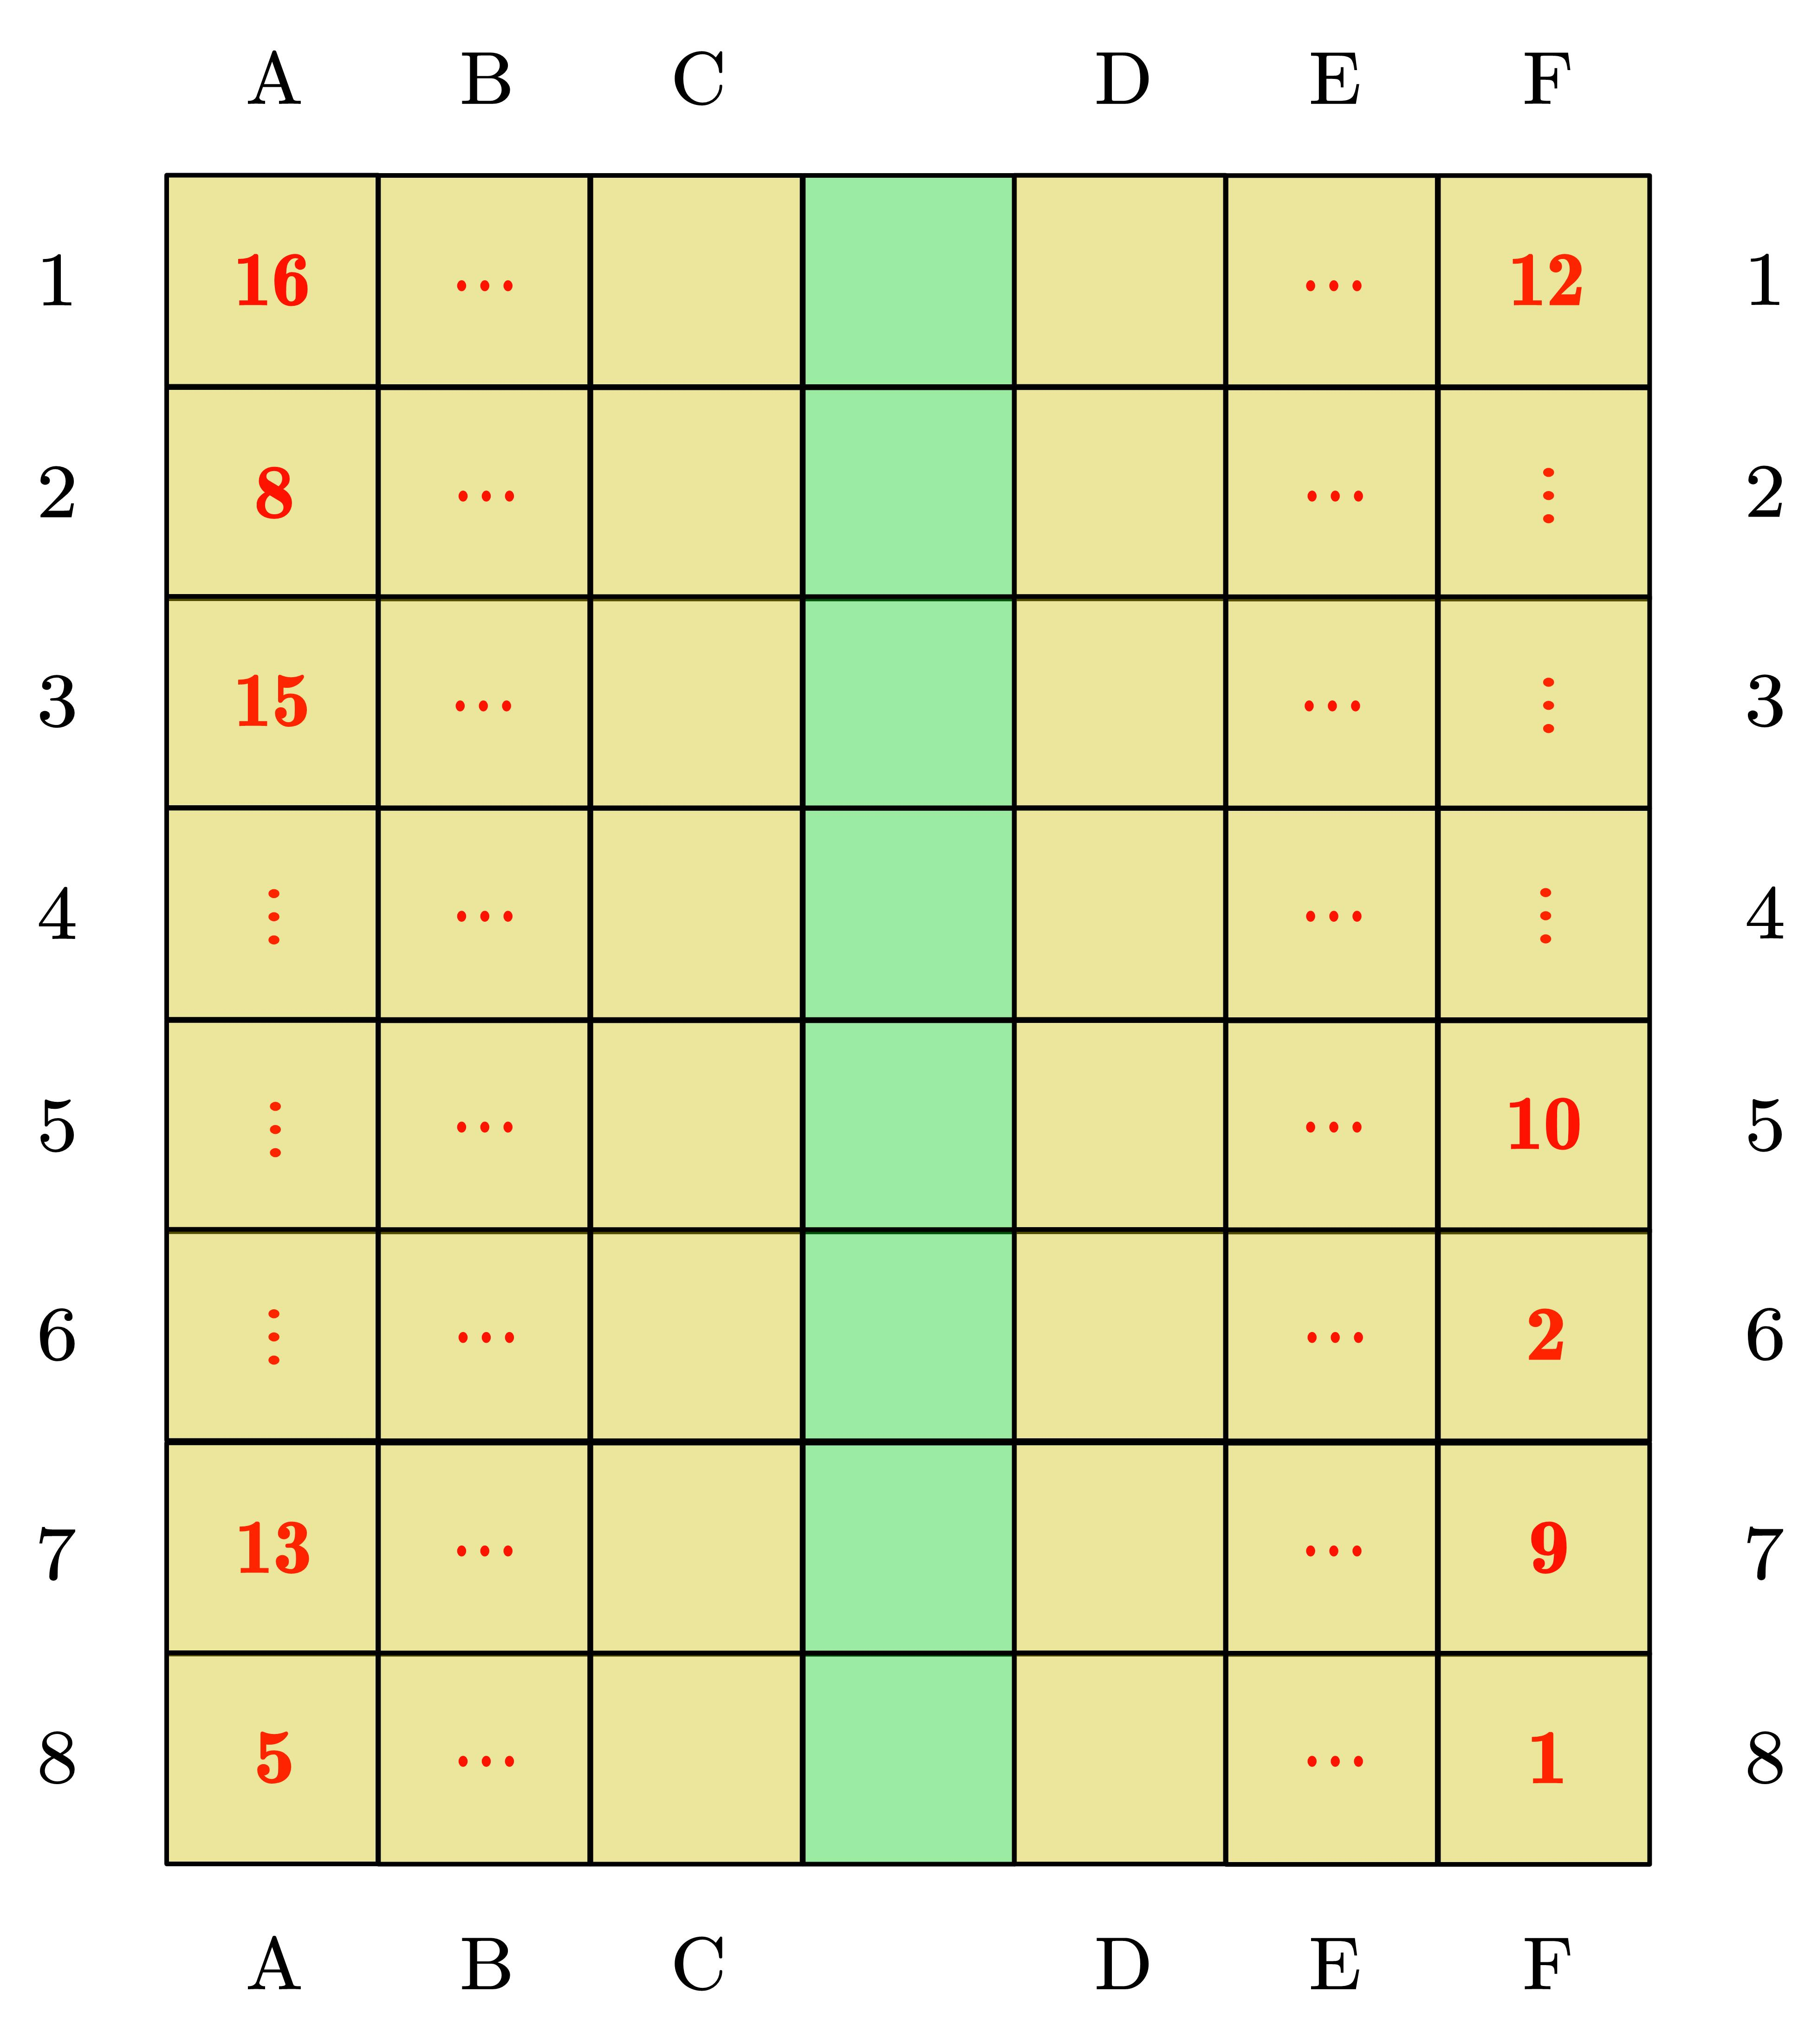
\includegraphics[height =4cm]{steffen1.jpg}
		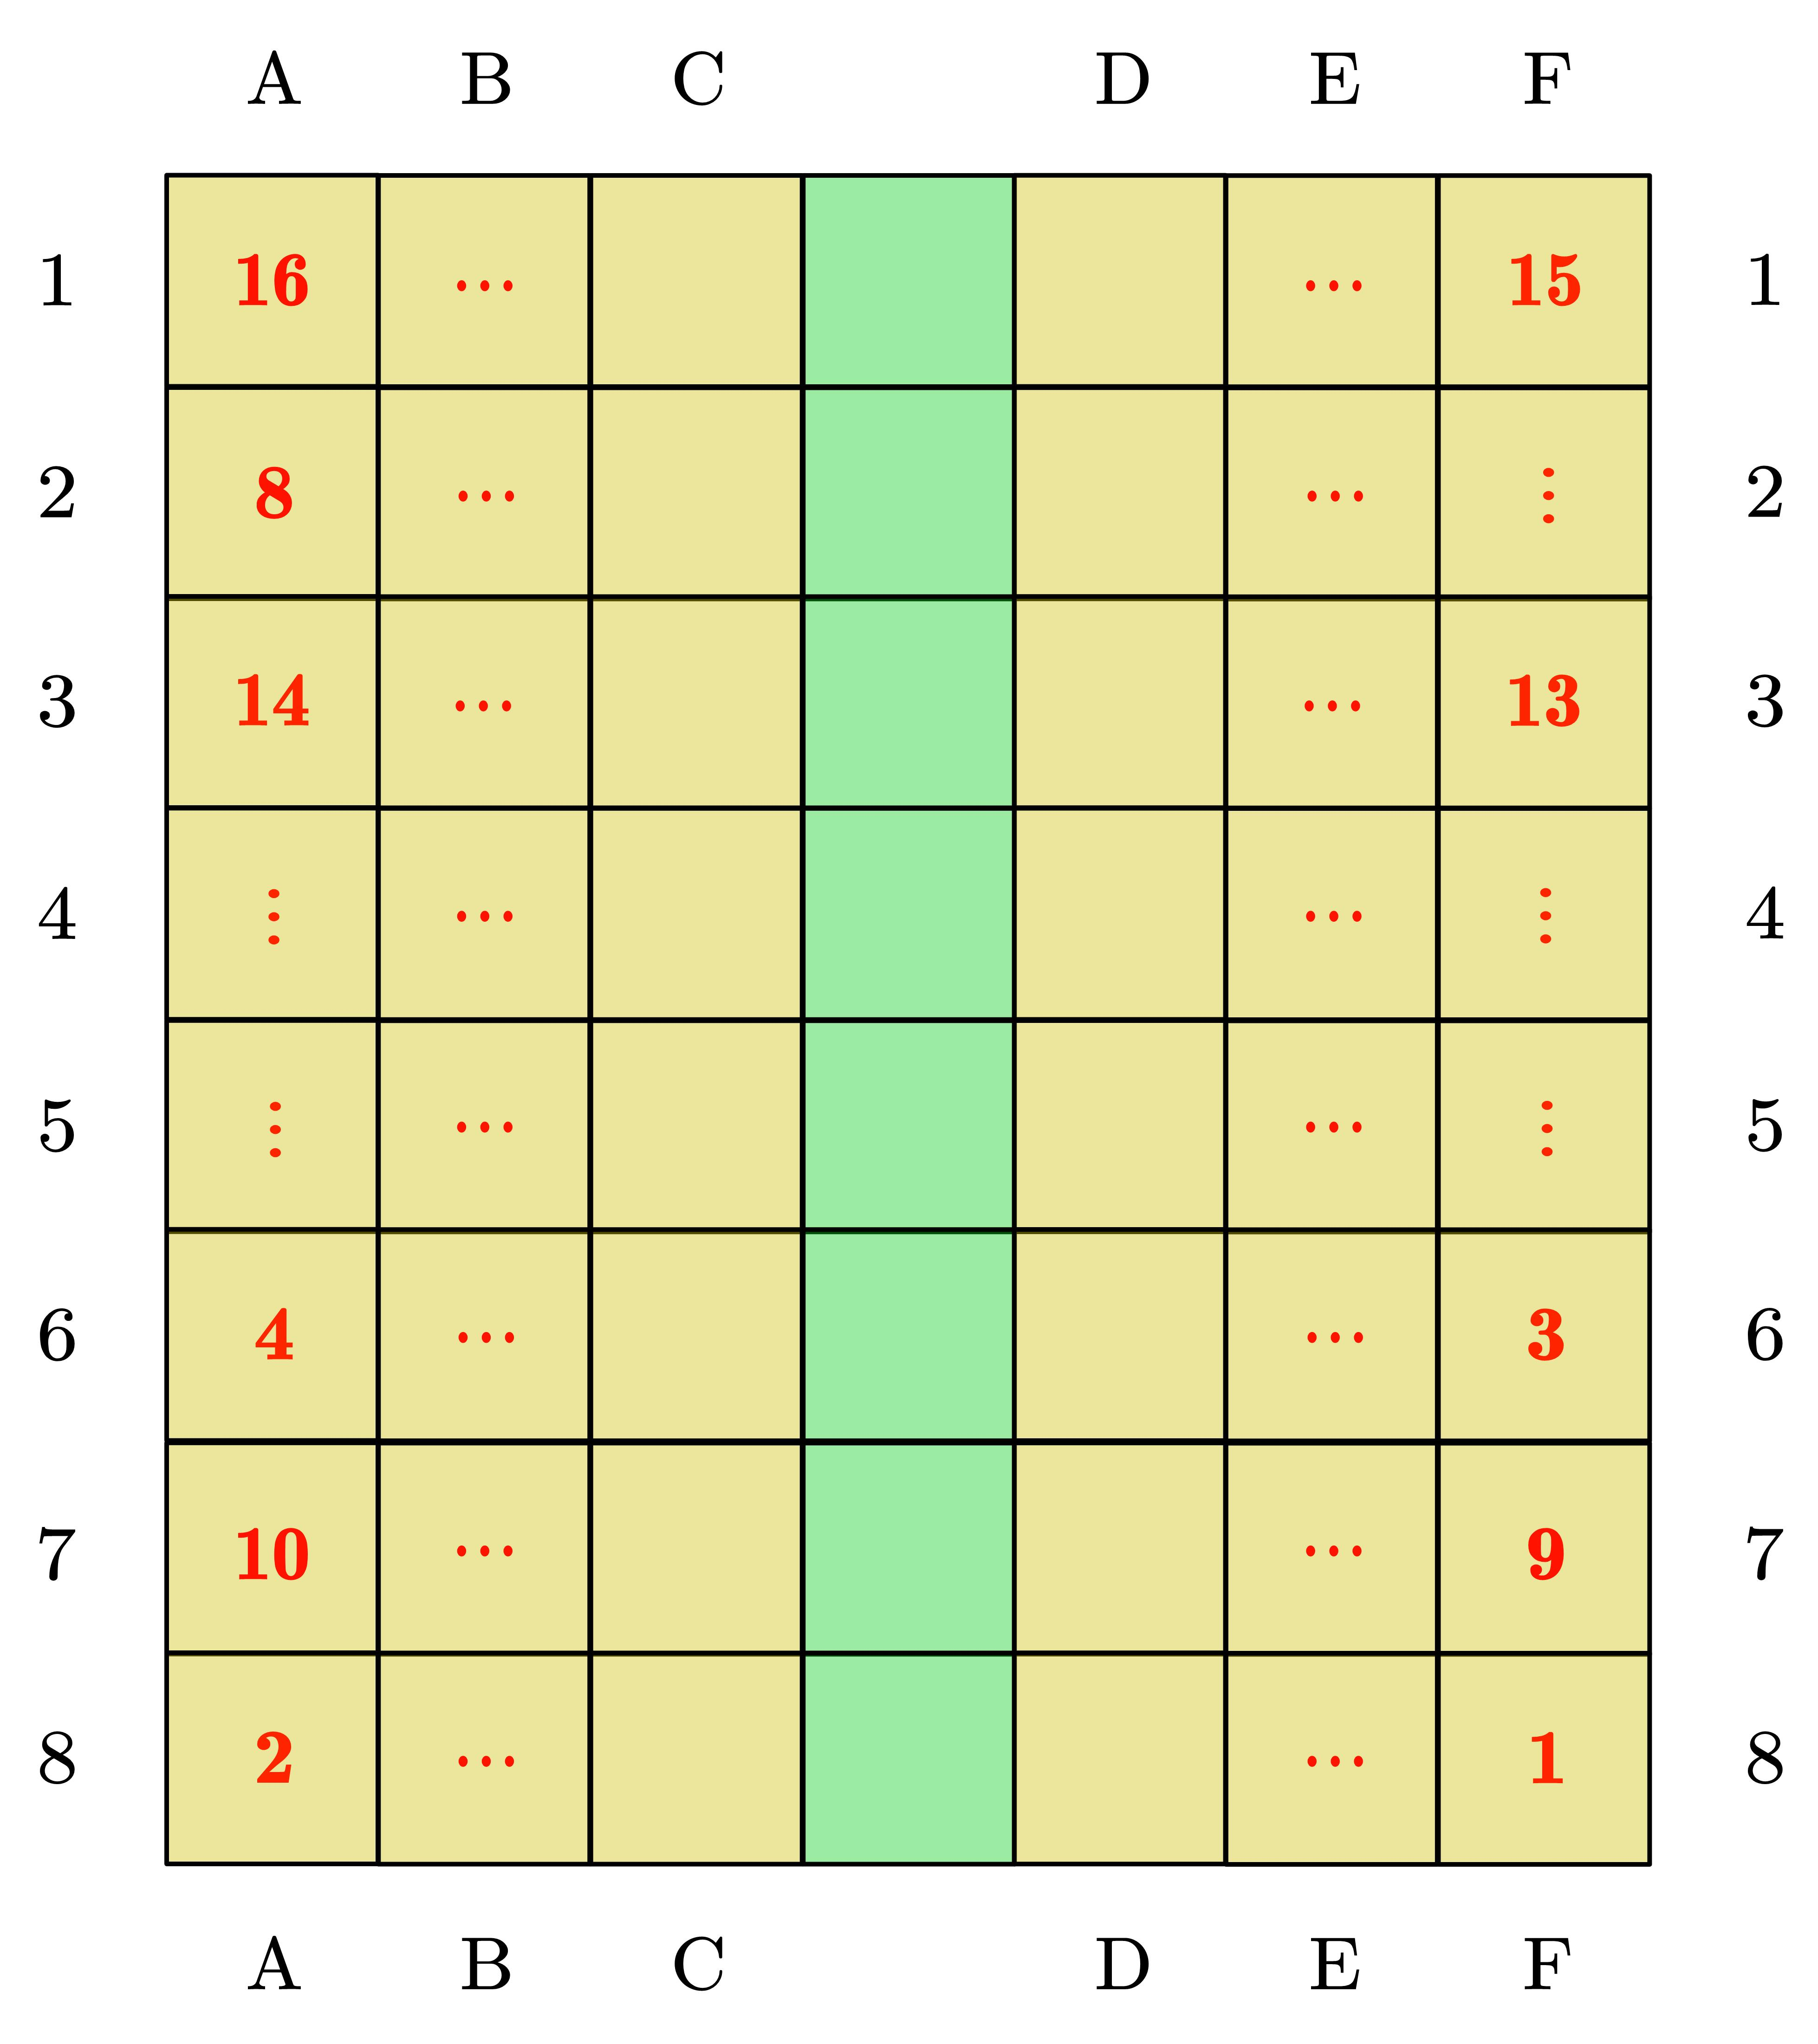
\includegraphics[height = 4cm]{steffen2.jpg}

		\small\textit{Fig. Two ideal boarding plans}
	\end{center}




	\section{Model B: Reoptimizing the strategy with passenger satisfaction}
	\subsection{Model Overview}
		In model A, we've found the pattern of the optimal model. However, it's also crucial to notice the fact that in this model, passengers in the same row are highly separated. This would, as a result, greatly increase the dissatisfaction among families where parents should have been placed adjacent to their children in the queue. Therefore, in model B, we'll comprehensively consider passengers' satisfaction and therefore yield the most \textit{user-friendly} boarding strategy.
	\subsection{Notation}
	\begin{center}
	\begin{tabular}{|l|l|}
		\hline
		$\alpha_\text{satisfy}(A)$&satisfactory index of passenger $A$\\
		\hline
		$\alpha$&satisfactory index of a whole plan\\
		\hline
		$k_1$, $k_2$, $k_3$&constanrts describing the weight of each factor\\
		\hline
		$D_i$&variance of the boarding time of the passenger whose seat is in the $i^\text{th}$ row\\
		\hline
		\(\xi\left(A\right)\) & the total time passenger A needs to offer his/her seat\\
		\hline
	\end{tabular}
	\end{center}
	\subsection{Satisfactory Index}
	In this part, we mainly dicuss which methods can best satsify the passengers.

	\begin{itemize}
		\item \defword{Queueing}: The longer a customer stays in a queue,
	\end{itemize}
	To make our result more precise, we define a series of constants ($k_1$, $k_2$ and $k_3$) to determine the factors' weight. Currently, the value of $k_1$, $k_2$ and $k_3$ are respectively 1, 5 and 1. The reason is that in real life experience, the process of offering seats for others is more unsatisfactory than that of waiting in the queue, but not so much. As a result, we define $k_2$ five times as big as $k_1$. The unsatisfaction caused by split groups can also be big, but considering that the proportion of group passengers are relatively small, we define $k_3$ the same as $k_1$.

	Together we find out the definition of satisfactory factory of a certain passenger, which is:

	$$\alpha_\text{satisfy}(A)=k_1\cdot \tau_j(A)+k_2\cdot\xi\left(A\right)+D$$

	To sum up, we can get the satisfactory index of a whole plan. The bigger $\alpha$ is, the less satisfied the passengers are and the less possible the plan can be applied to daily life.
	$$\alpha=\dfrac{\sum\limits_{A\in P} \alpha_\text{satisfy}(A)}{N}$$
	\subsection{Different Ways of Boarding}
	In this part, we will introduce some common ways of boarding and find out their effiencies based on the $\Gamma$ and $\alpha_\text{satisfy}$ of it. The picture below shows the plane we use to assess the boarding process.

	\begin{center}
		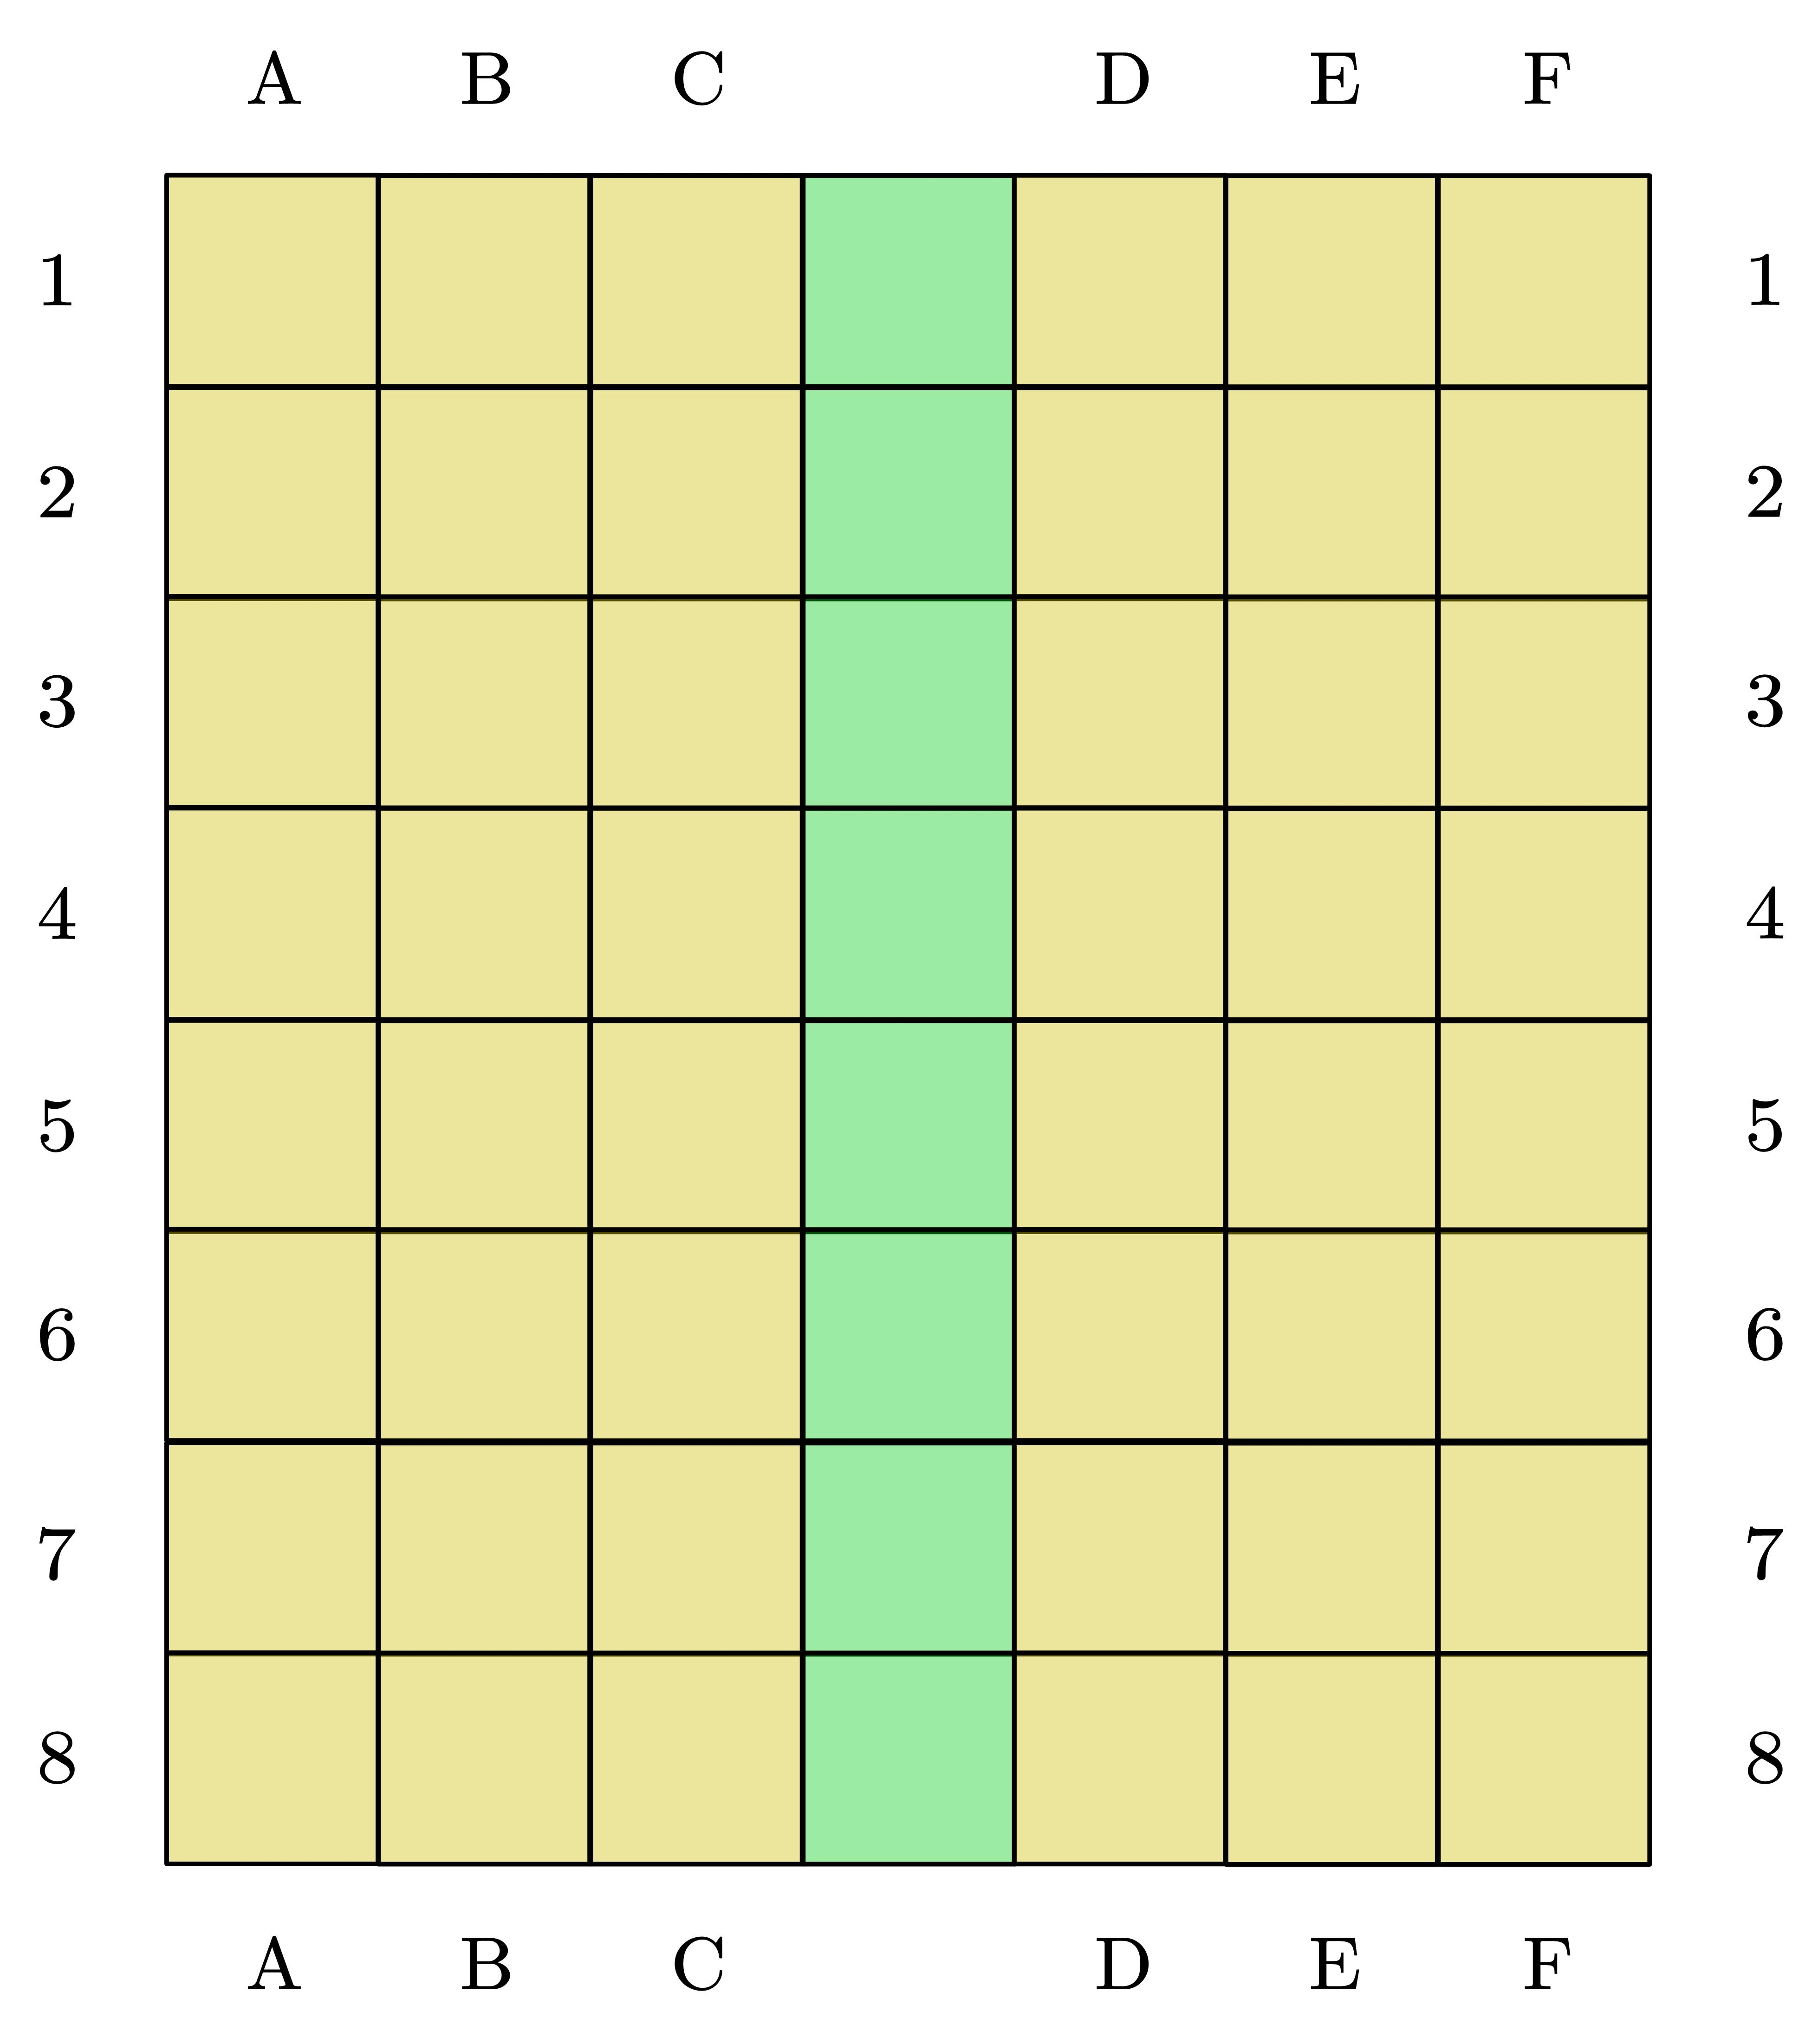
\includegraphics[height=5cm]{planeempty.jpg}

		\small \textit{Fig. Basic plane type}
	\end{center}

	The first method is based on row numbers. People enter the plane according to their row number. The plane is divided into several crosswide sections.or example, in one plan, a passenger with a smaller row number can be seated earlier and in other plane, he will enter later. We conclude these types as "front to back" and "backk to front".

	The second method is to board on plane according to their seat positions. The plane is divided into lengthways sections in this strategy. This time, passengers whose seats are A or F may enter the plane first to minimize the time wasted in offering seats.

	The third method is let the passengers get onboard uninstructedly, which means that the boarding order is random. The picture below shows the whole process of this boarding method.
	\begin{center}
		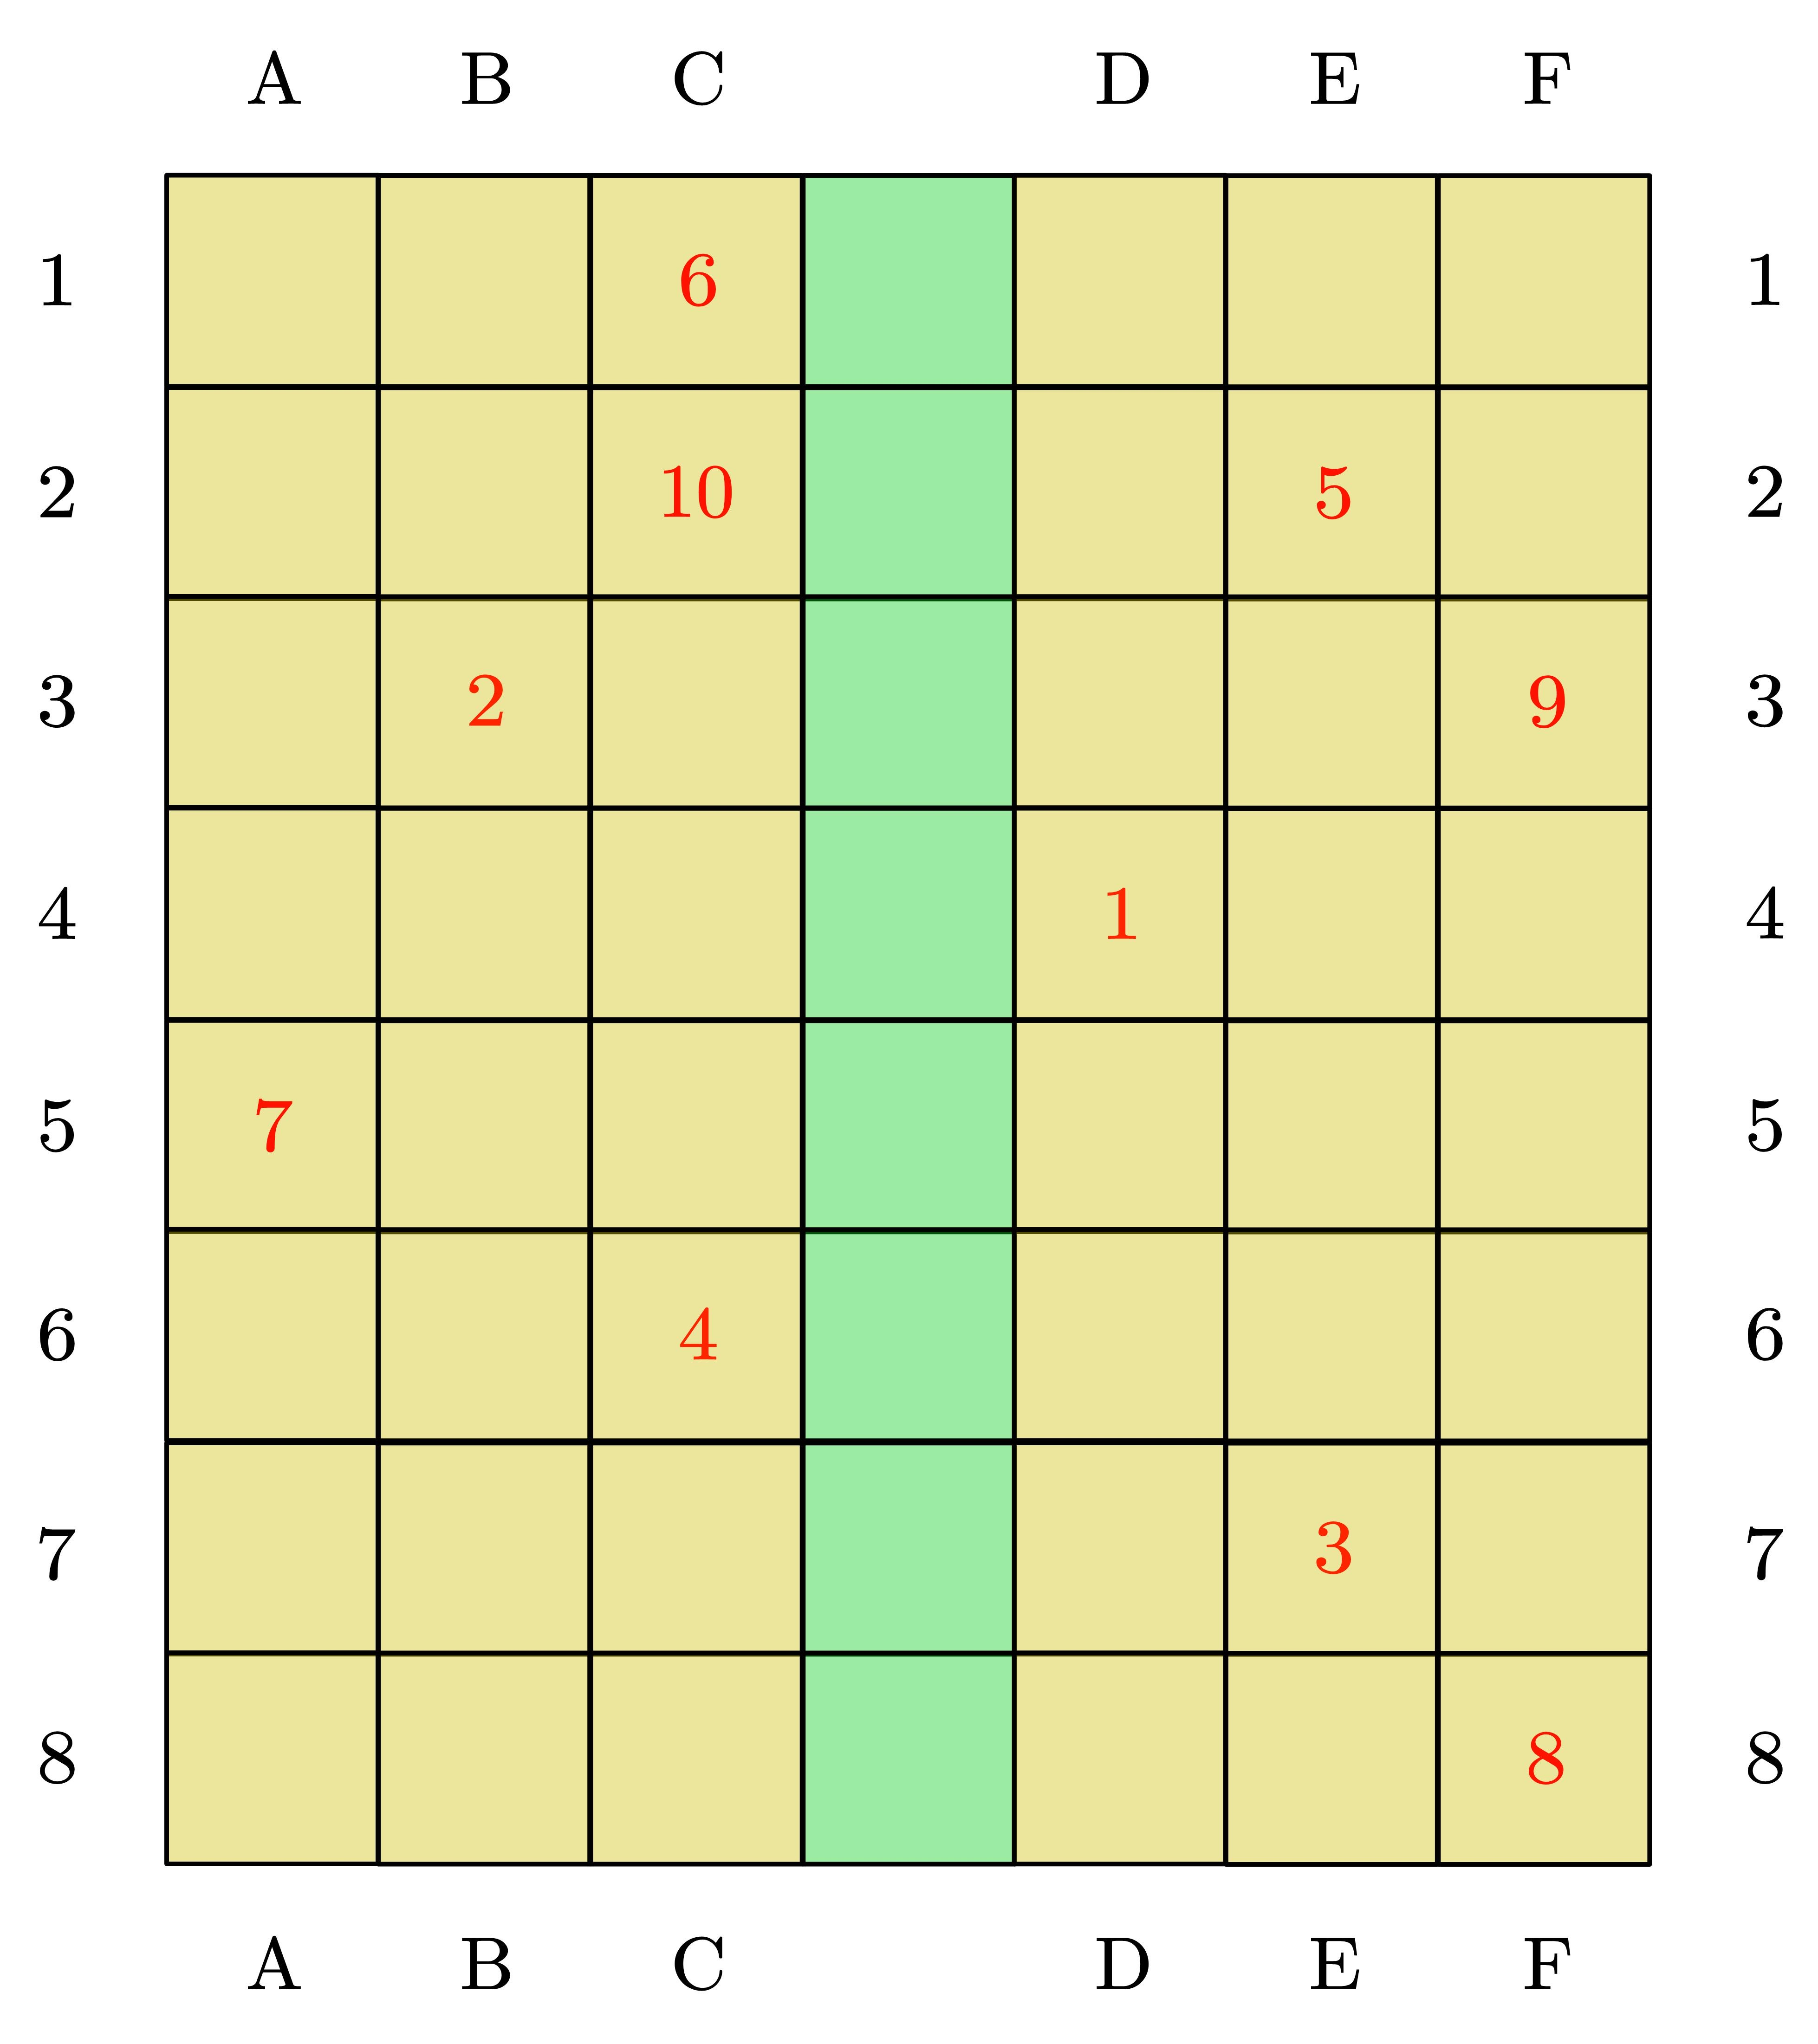
\includegraphics[height=5cm]{planerandom.jpg}

		\small \textit{Fig. Plane constructed randomly}
	\end{center}
	The dour pictures below can effectively explain the methods.

	\begin{center}
		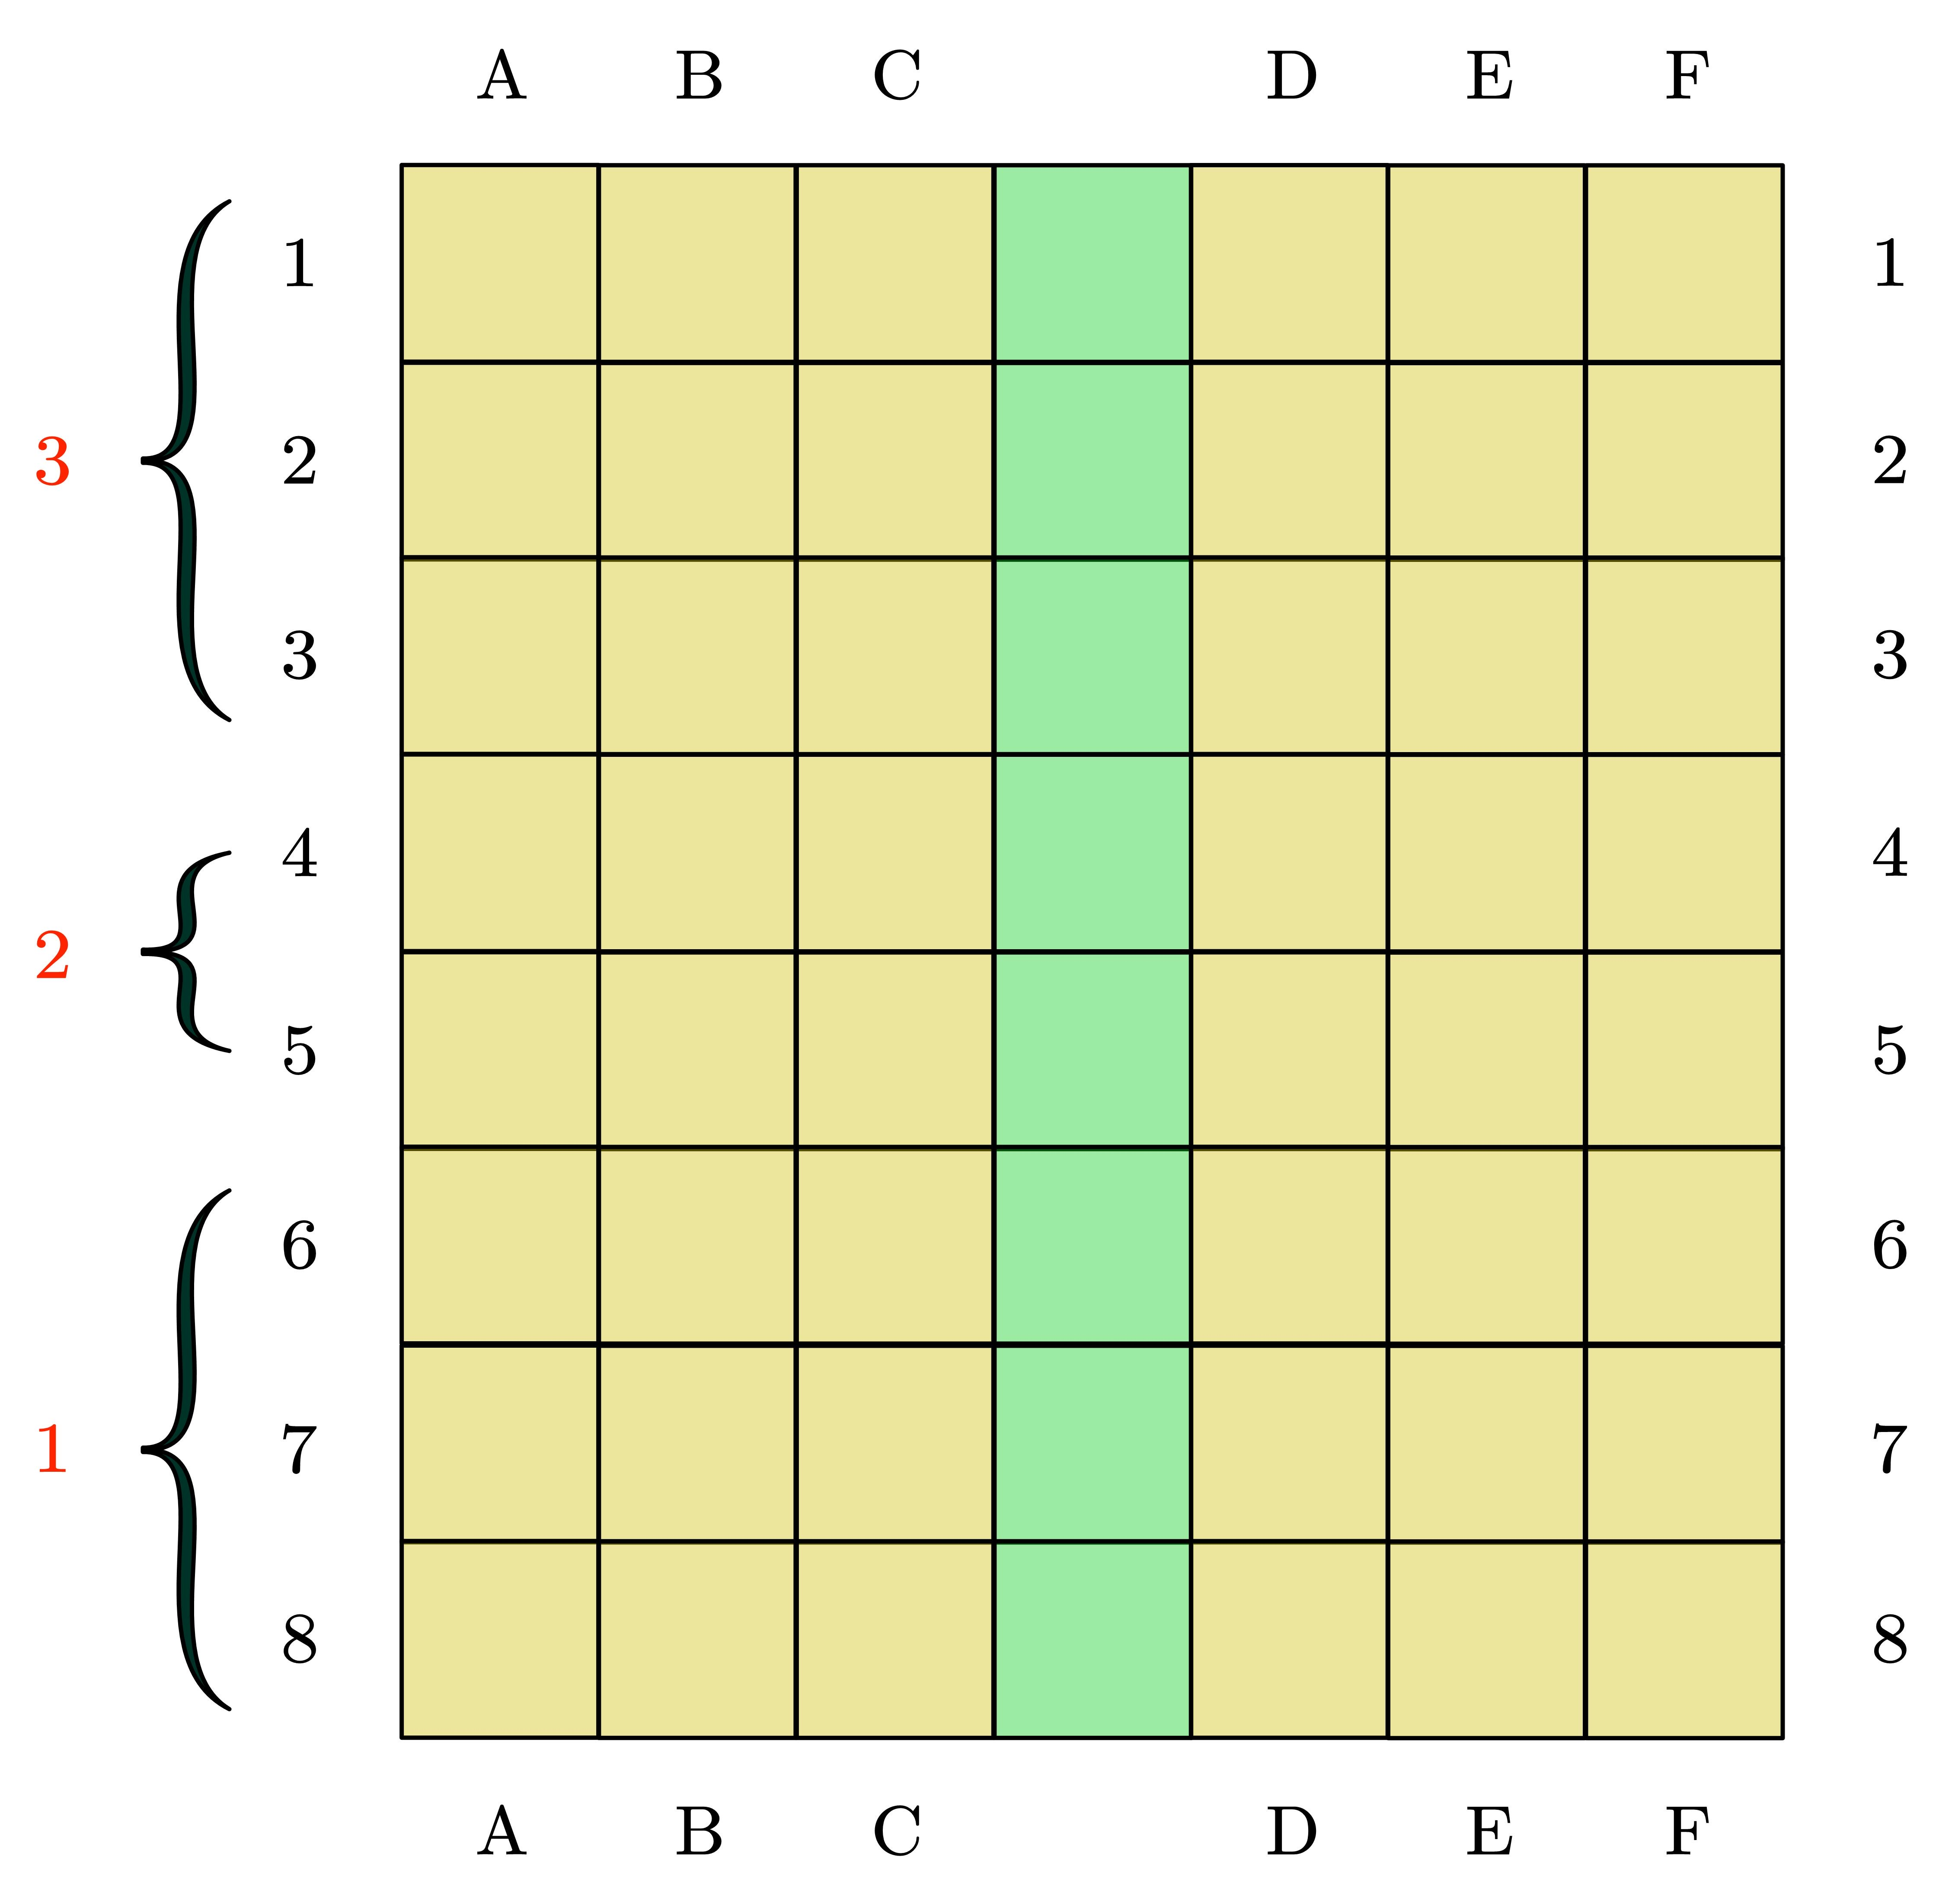
\includegraphics[height=5cm]{planerow1.jpg}
		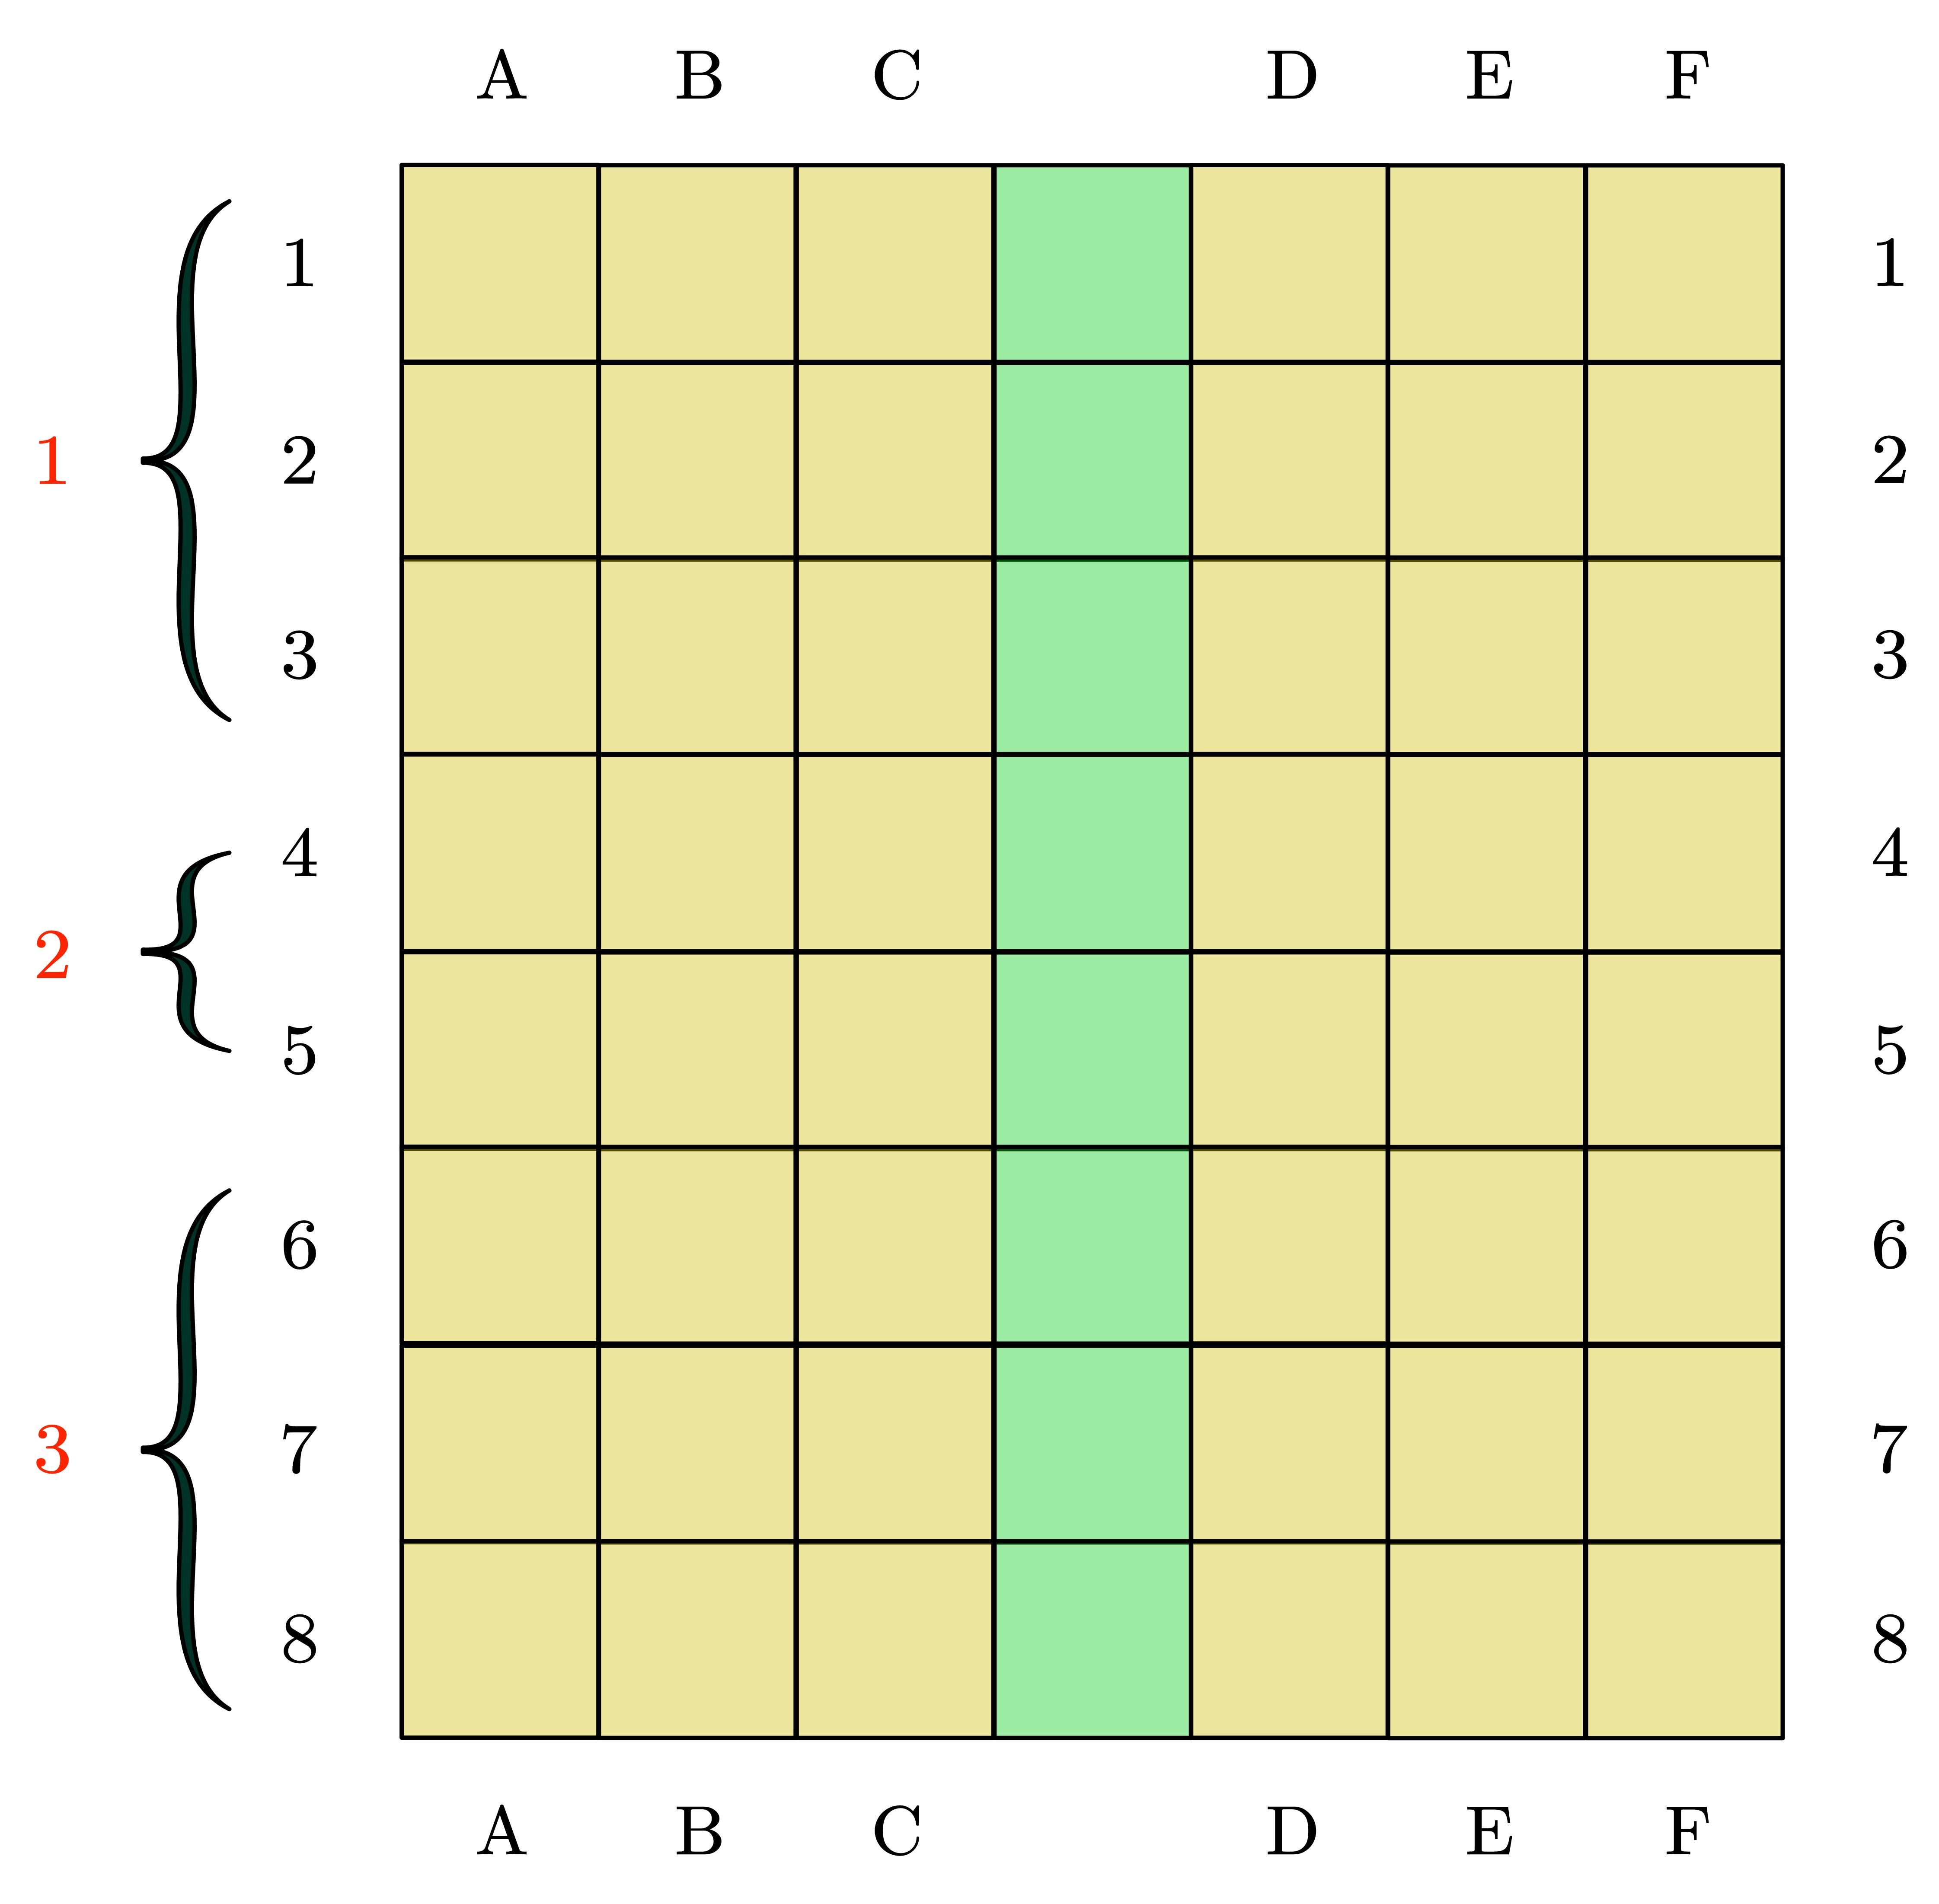
\includegraphics[height=5cm]{planerow2.jpg}\\
		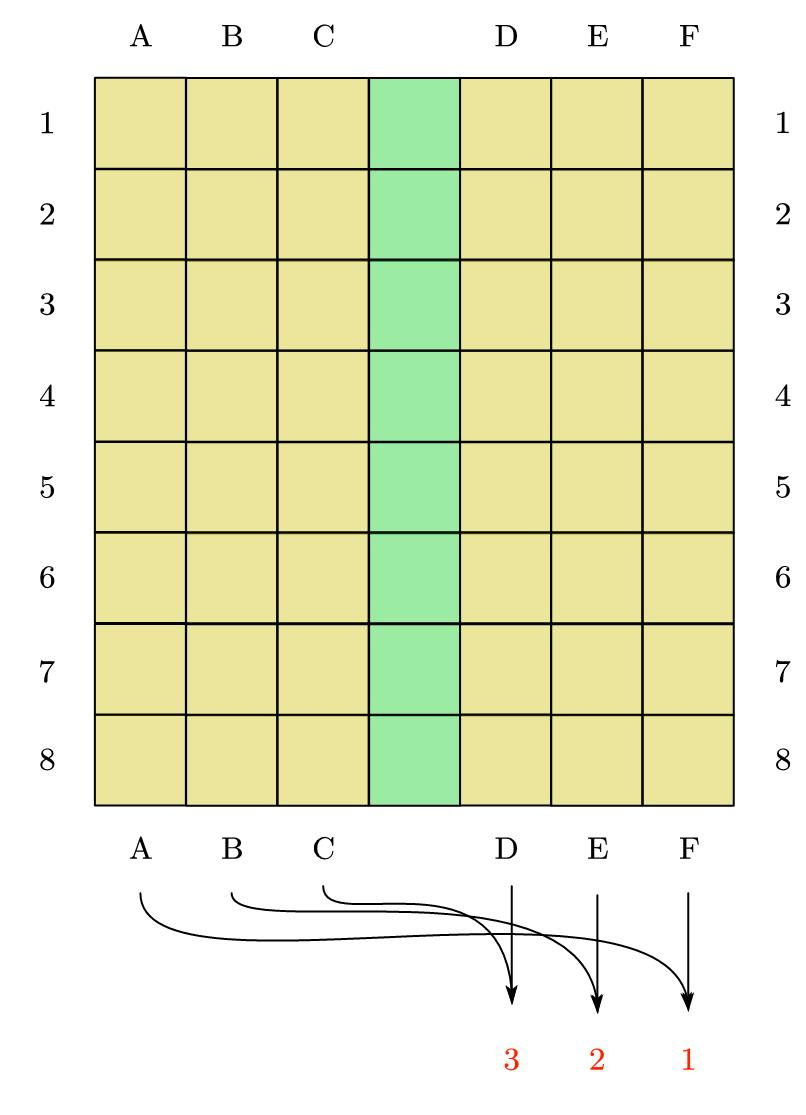
\includegraphics[height=5cm]{wdmd.jpg}
		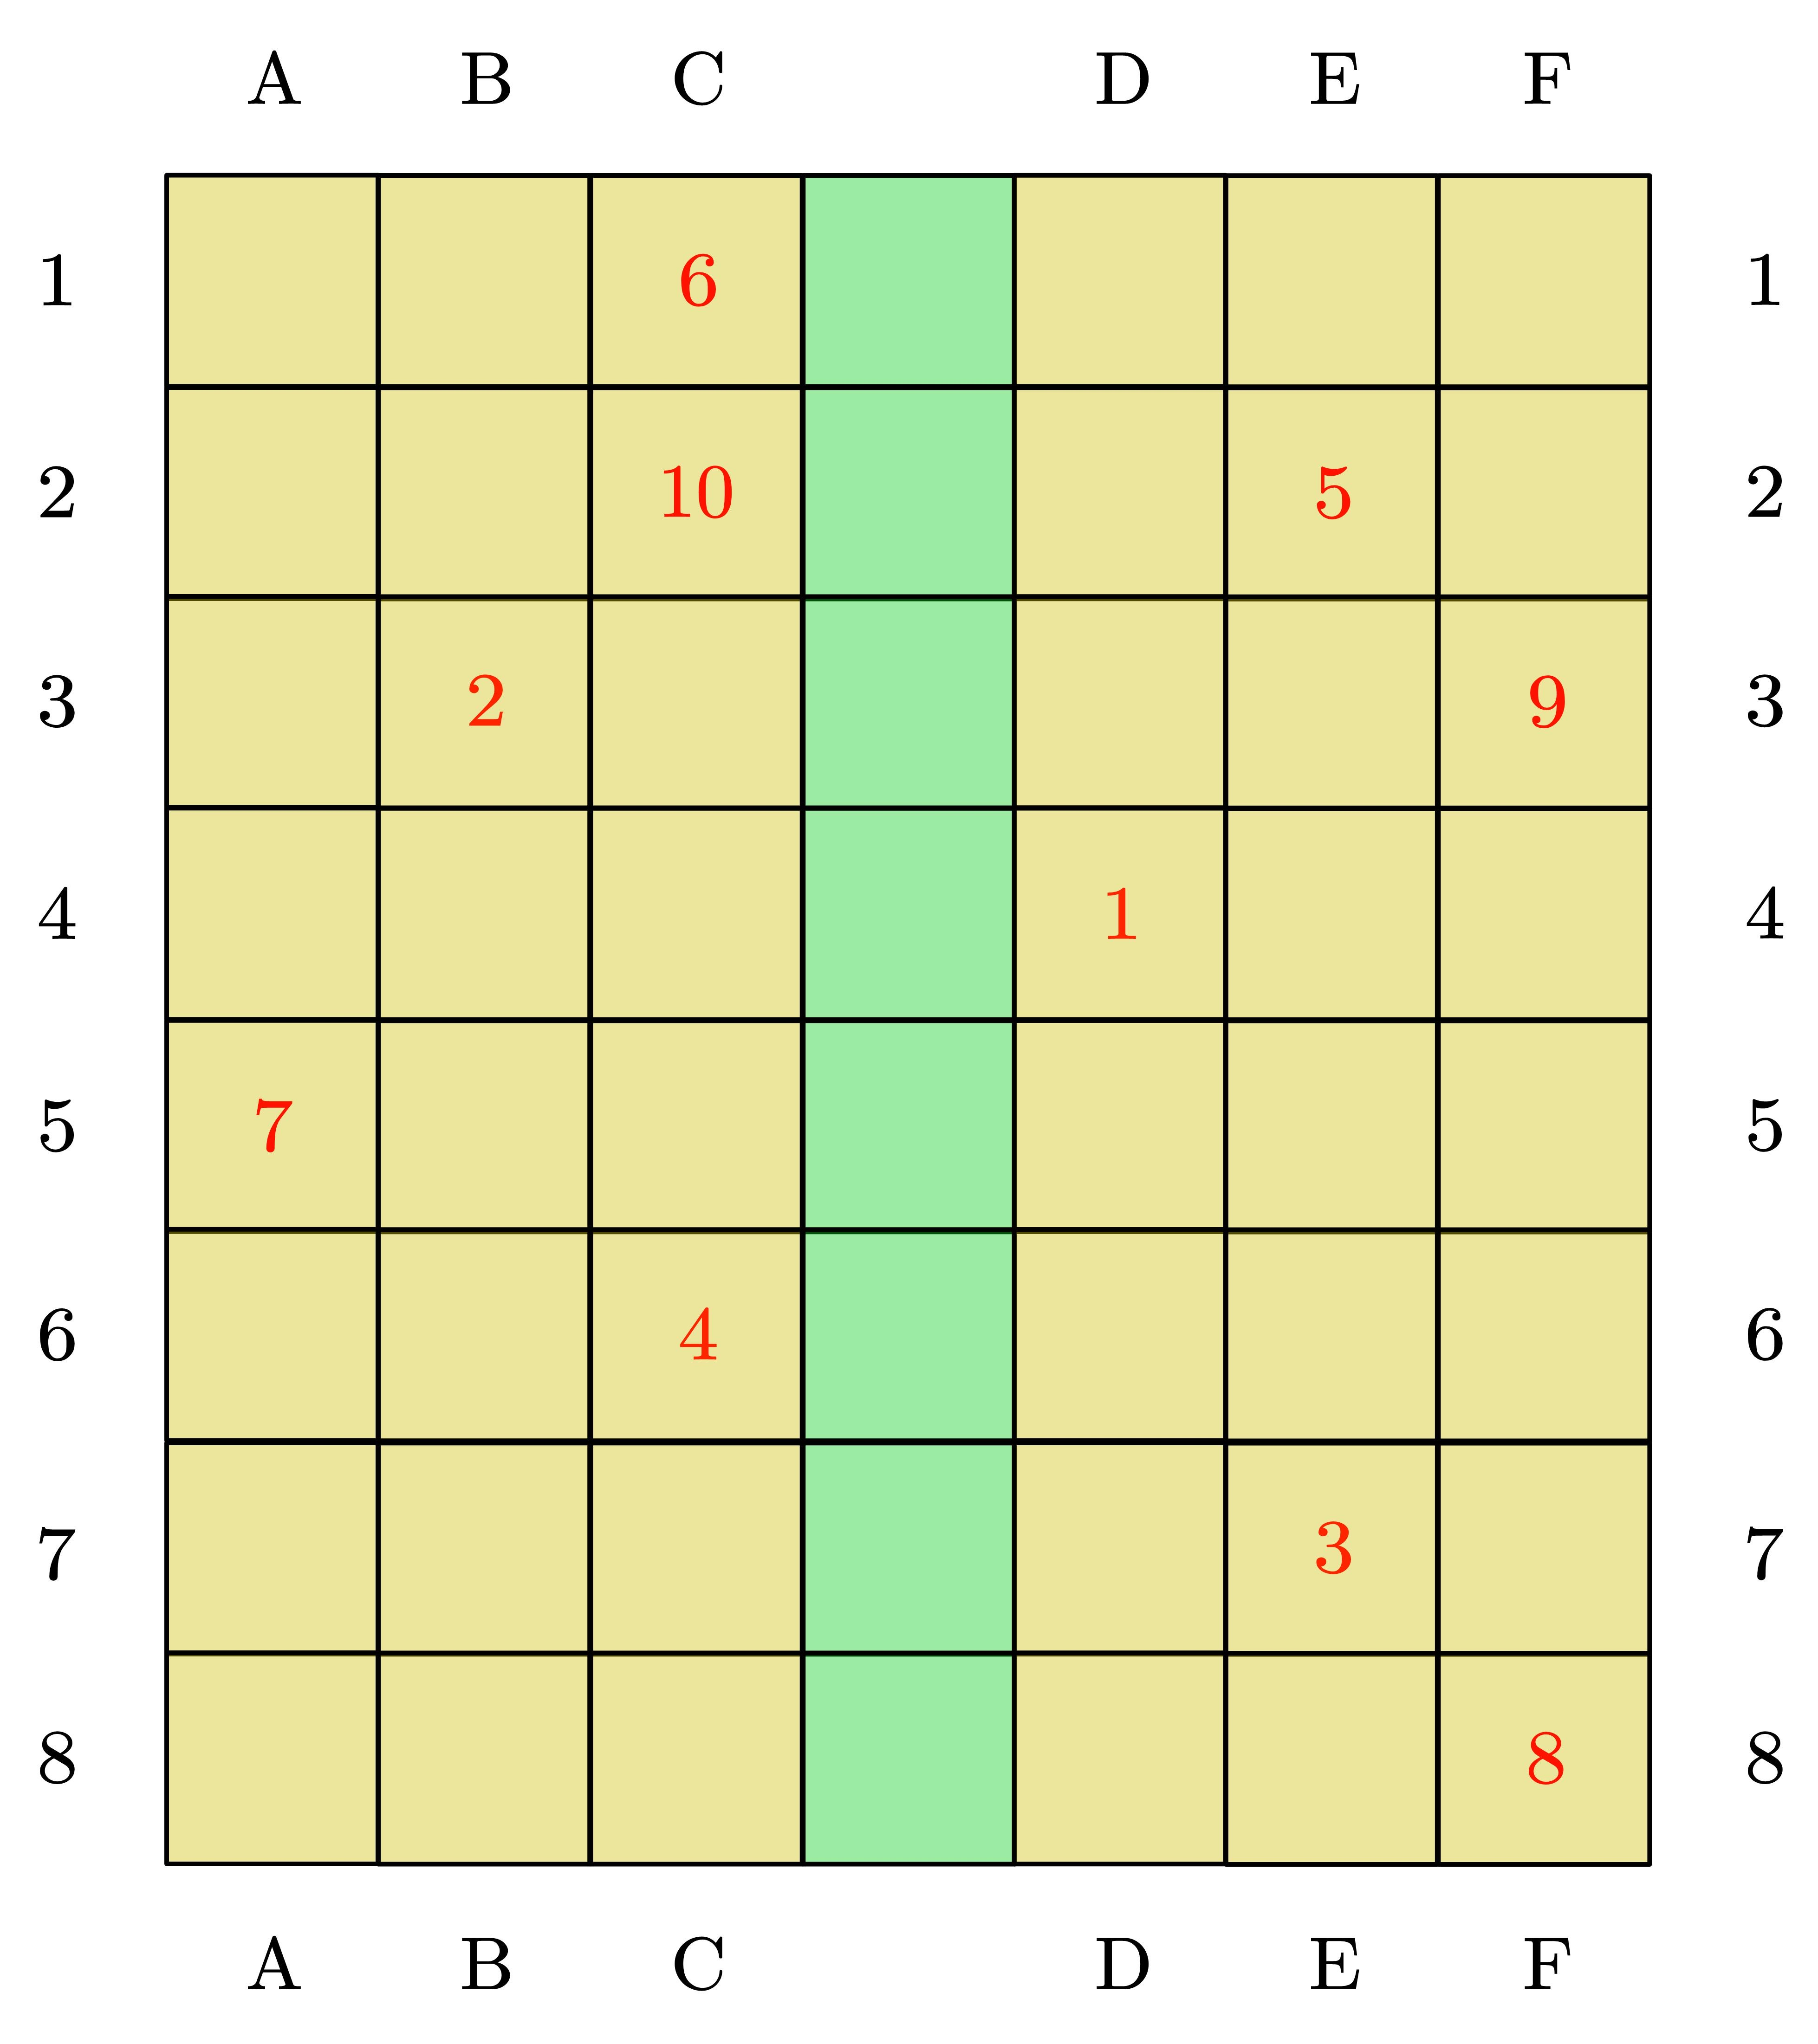
\includegraphics[height=5cm]{planerandom.jpg}

		\small \textit{Fig. Four different methods}
	\end{center}

	In conclusion, we can draw a form to compare $\Gamma$ and $\alpha_\text{satisfy}$.

	\begin{center}
	\begin{tabular}{||l|l|l||}
		\hline
		Boarding type&Time step required&$\alpha_\text{satisfy}$\\
		\hline
		From front to back&5029&~\\
		From back to front&4092&~\\
		Window middle aisle&4347&~\\
		Random Boarding&4409&~\\
		\hline
	\end{tabular}
	\end{center}
	From this we can find that, boarding from front to back need the maximum time, which means that it may not be so reasonable when applied to daily life. Boarding from back to front, on the other hand, is the most  efficient time. However, its easy to find that the difference between the three latter methods is not a big number, which we will explore further in \defword{Sensitivity Analysis}.

	Apart from the common ways used by air executives introduced above, we also figure out some plans of our own and proposed by others. The strategies are as follow.
	\begin{itemize}
		\item The first plan introduced is the Steffen Mode\cite{steffen}. In this mode,  passengers will board the plane from the inner seat to the outer seat, from the rear to the front and in separate rows. Because the passengers sitting on the back and inside board first, there will be no queueing caused by the luggage of the front passengers and the situation that the outer passengers give up their seats for the inner passengers, which effectively reduces the waste of time caused by congestion and seat giving. At the same time, when boarding, passengers who put their luggage generally need to occupy the aisle next to two rows of seats. Therefore, it can be proved that sitting in separate rows is a seating method with the highest parallel efficiency, which can allow the most passengers to sit in parallel. Taken together, this shows that Steffen mode is a great boarding strategy. Here is a picture which explains the whole process:

		\item Another optimal boarding strategy is to divide the plane into six parts (demonstrated in the picture below). This strategy combine all the strengths together: it can perfectly reduced the time of offering seats, queueing and raise the passenger's satisfactory index. However, this may also lead to some other problems.

		\begin{center}
			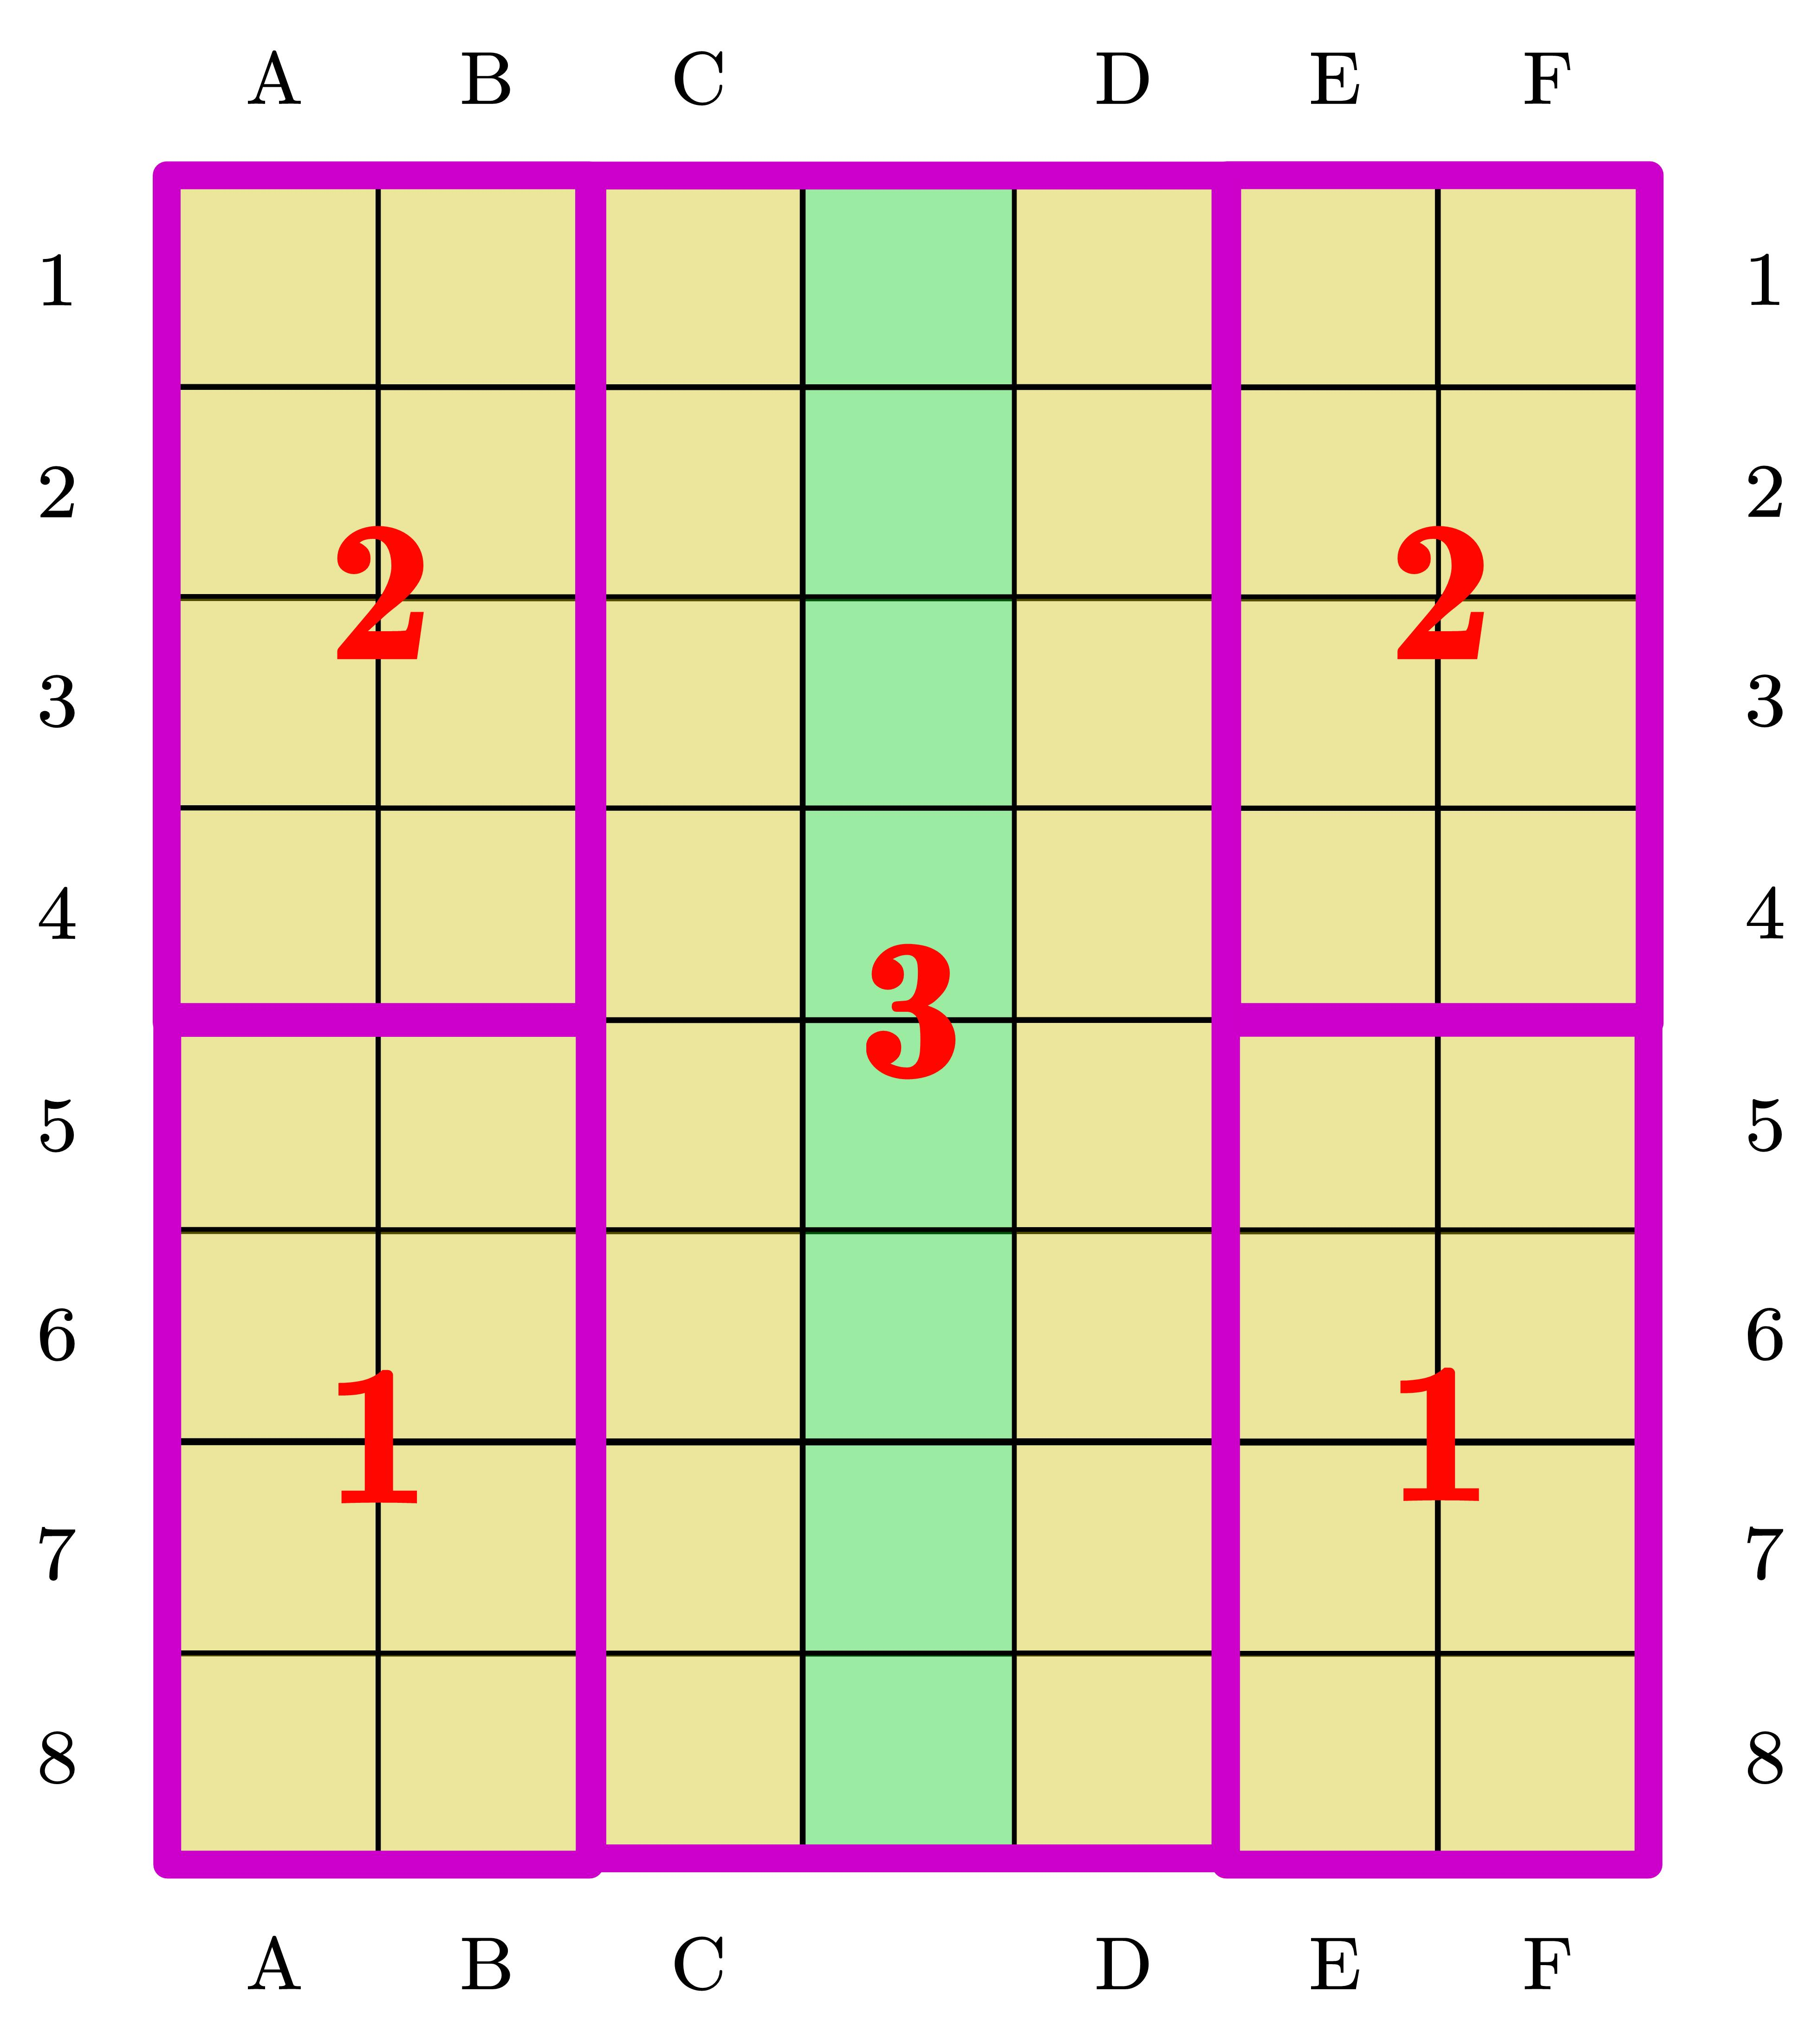
\includegraphics[height=5cm]{planeown.jpg}
		\end{center}
	\end{itemize}
	As previously mentioned, methods back-to-front and window-to-aisle are two great plans of boarding. Therefore, we decided to combine them and divide the back-to-front sections smaller. To be exact, the sections are rows, and now the passengers enter with sorted sequence. To prevent passengers from colliding with each other, passengers are seated every two rows and side by side. We did research and found a method by **Steffen XXX** [CITE].

	As mentioned, passengers are seated side by side, which means a row will be seated 6 times. Therefore, we considered seating the passengers on the same row together, which can let them put luggage and be seated simultaneously. After conducting both a calculation and simulation, we reached a conclusion that this way is faster than the original Steffen method.

	\section{Sensitivity Analysis}
	As mentioned in \defword{Background}, there are always passengers who don't follow the instructions. To make sure how much "destruction" they will cause to the boarding process.

	To define the effect, we introduce a variable $\alpha_\text{discompliance}$. It will define a certain passenger's behavior and it's generated randomly by programs. This can make our result more accurate.

	\begin{center}
	\begin{tabular}{||l|l|l||}
		\hline
		Boarding type&Time step required before&Time step required now\\
		\hline
		From front to back&5029&5298\\
		\hline
	\end{tabular}
	\end{center}
	\begin{center}
		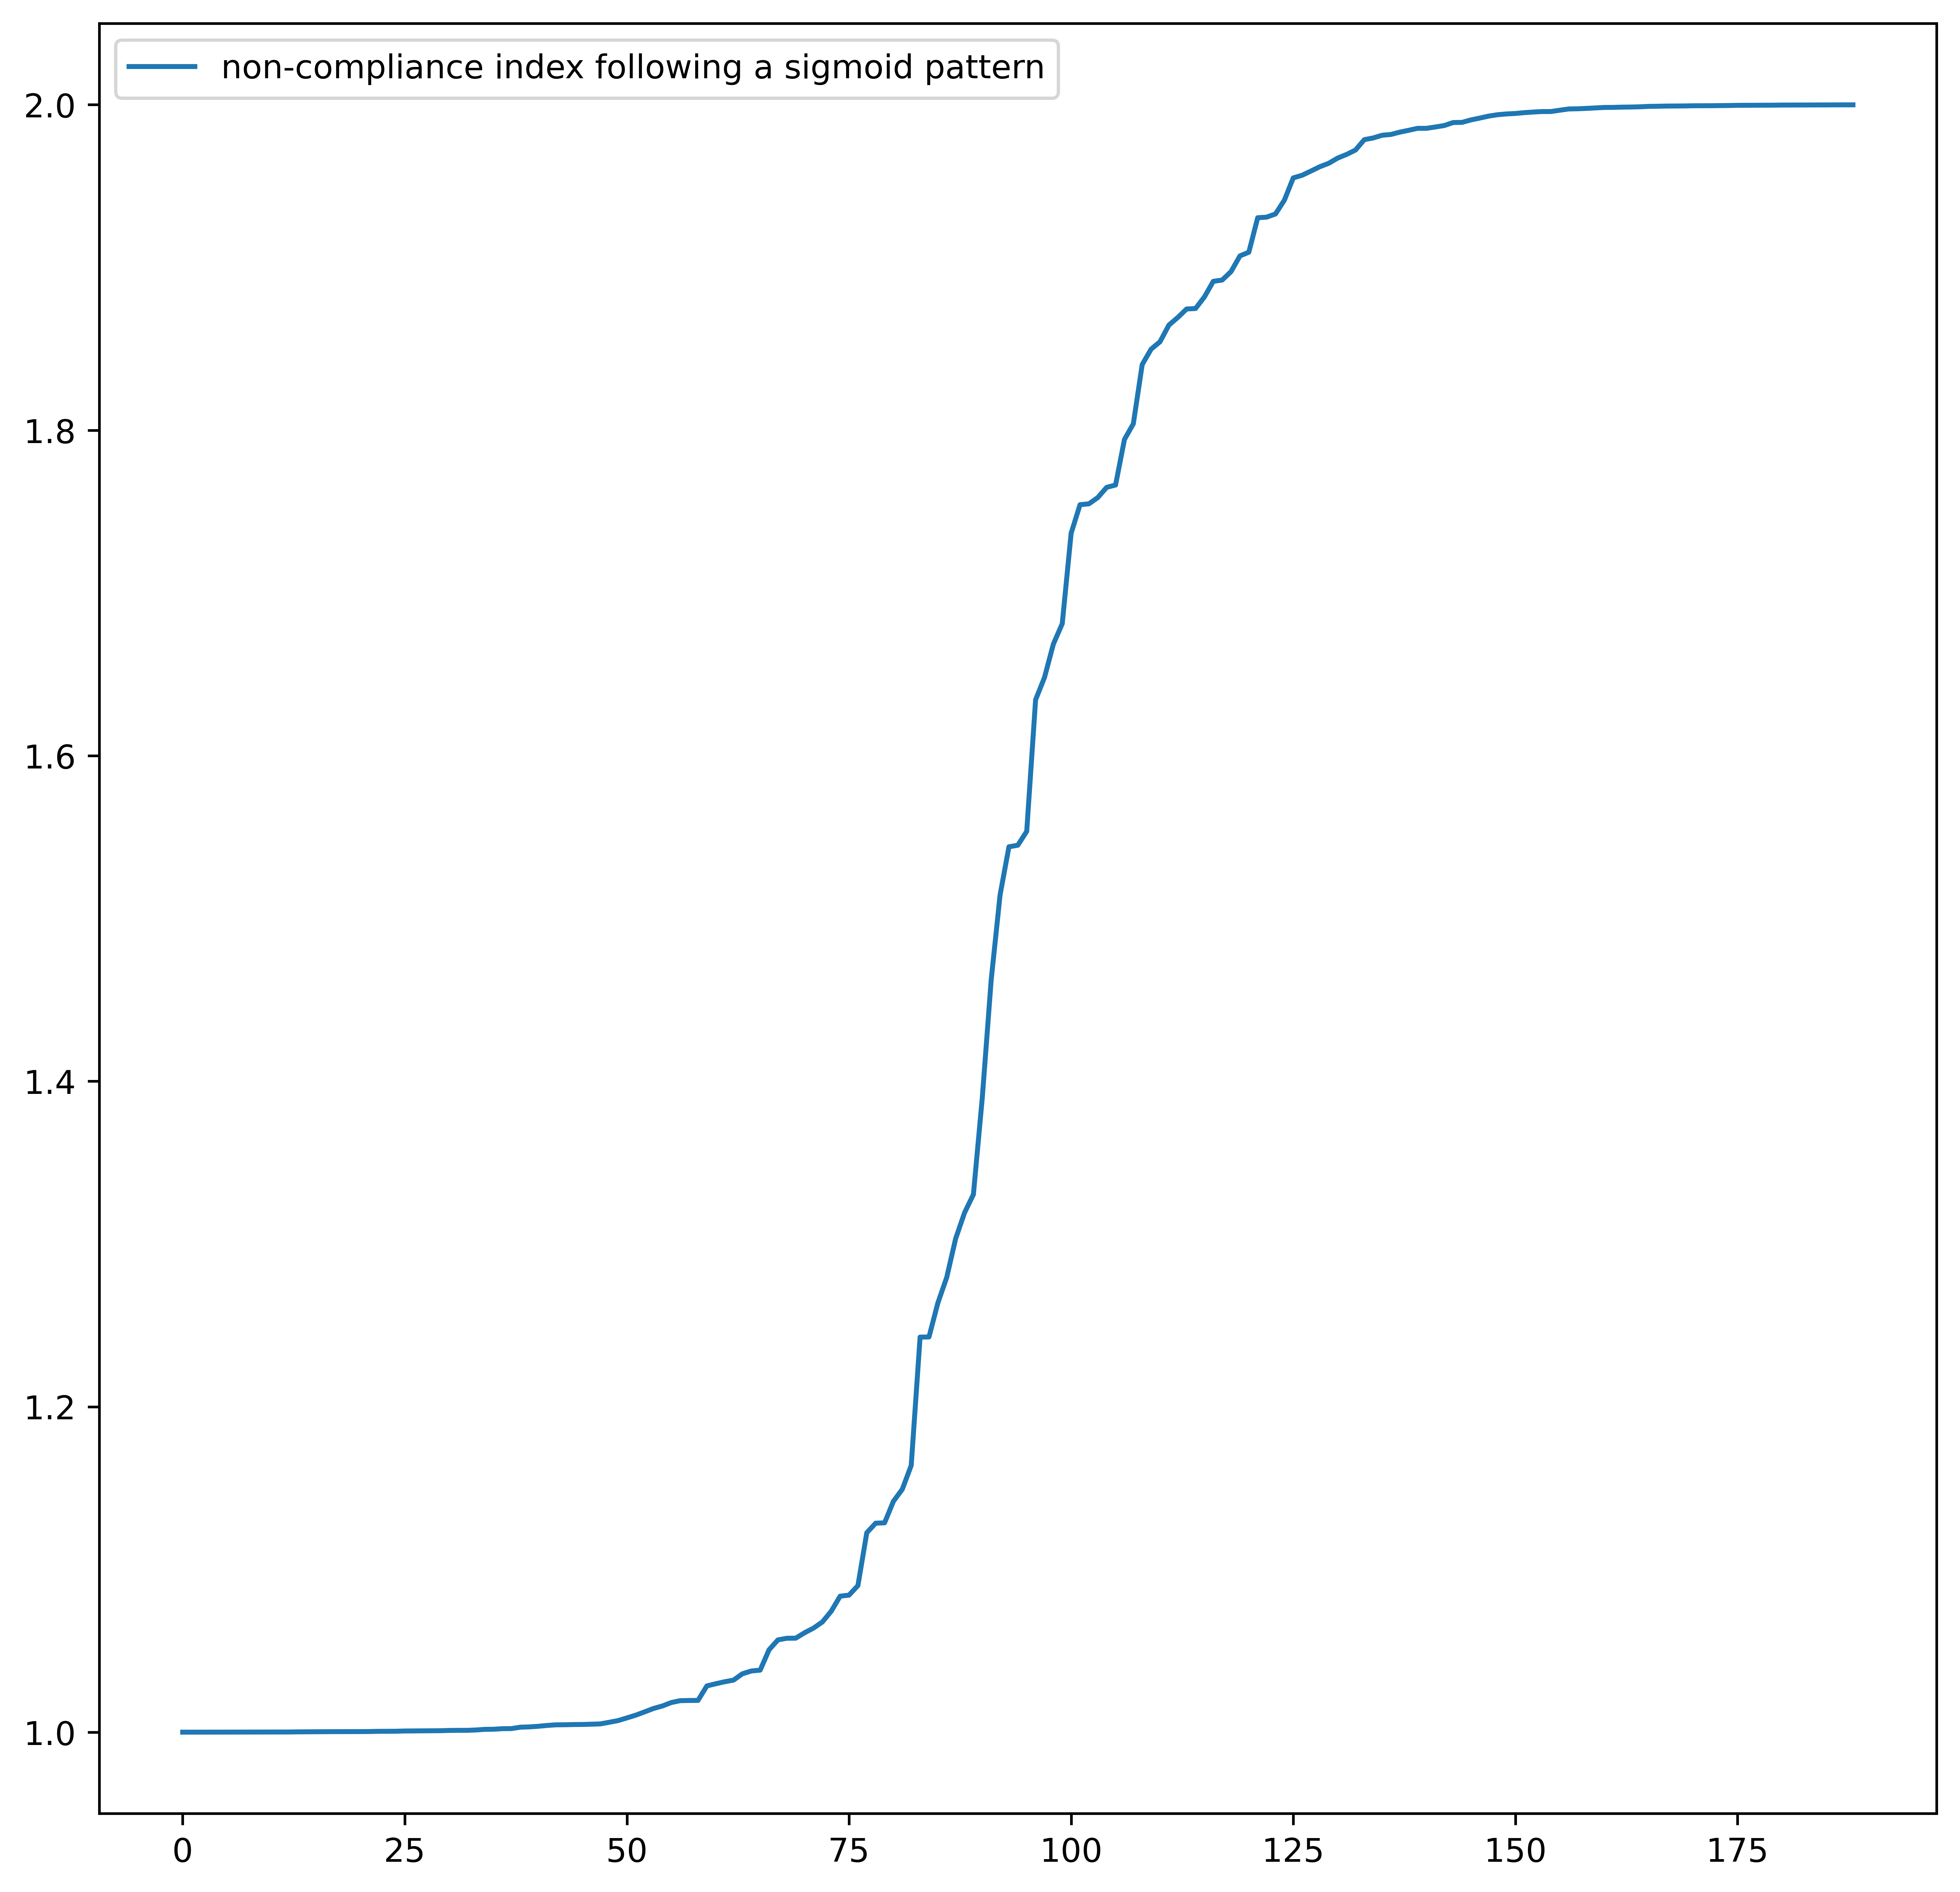
\includegraphics[width=6cm]{sigmoid.png}

		\small \textit{Fig. }
	\end{center}
	\section{Examining the Results}
	\subsection{Model Overview}
	In this model, we will apply our model to the images given by \# (The pictures will be shown in the next section) and find out the best strategy to them seperately. Later, we will give a brief advice about the the boarding plan. In addtion, we will list out two boarding plan that may also facilitate the air agency complete their mission and find out the efficiency of them based on our model.
	\subsection{Flying Wings}
	Flying  wings is a special kind of plane. Different from others, it's especially spacious and can accomodate a great number of people. It's shape is shown below. As can be seen in the graphics, we divide the plane into four parts and we will calculate the time used seperately.

	Though we define the plane into several rectangle cells, passengers can still travel in arctangles in this kind of plane. We can find that:

	$$\left| s_{\mathrm{prev}}-s_{\mathrm{now}} \right|=\left| d\sqrt{x^2+\left( \frac{7}{2}d \right) ^2}-\left( x+\frac{7}{2}d \right) d \right|
	\\
	\le \left| d\sqrt{l^2+\left( \frac{7}{2}d \right) ^2}-\left( l+\frac{7}{2}d \right) d \right|
	\\
	=\frac{18-2\sqrt{53}}{5}\approx 0.688\mathrm{m}
	\\$$

	\begin{center}
		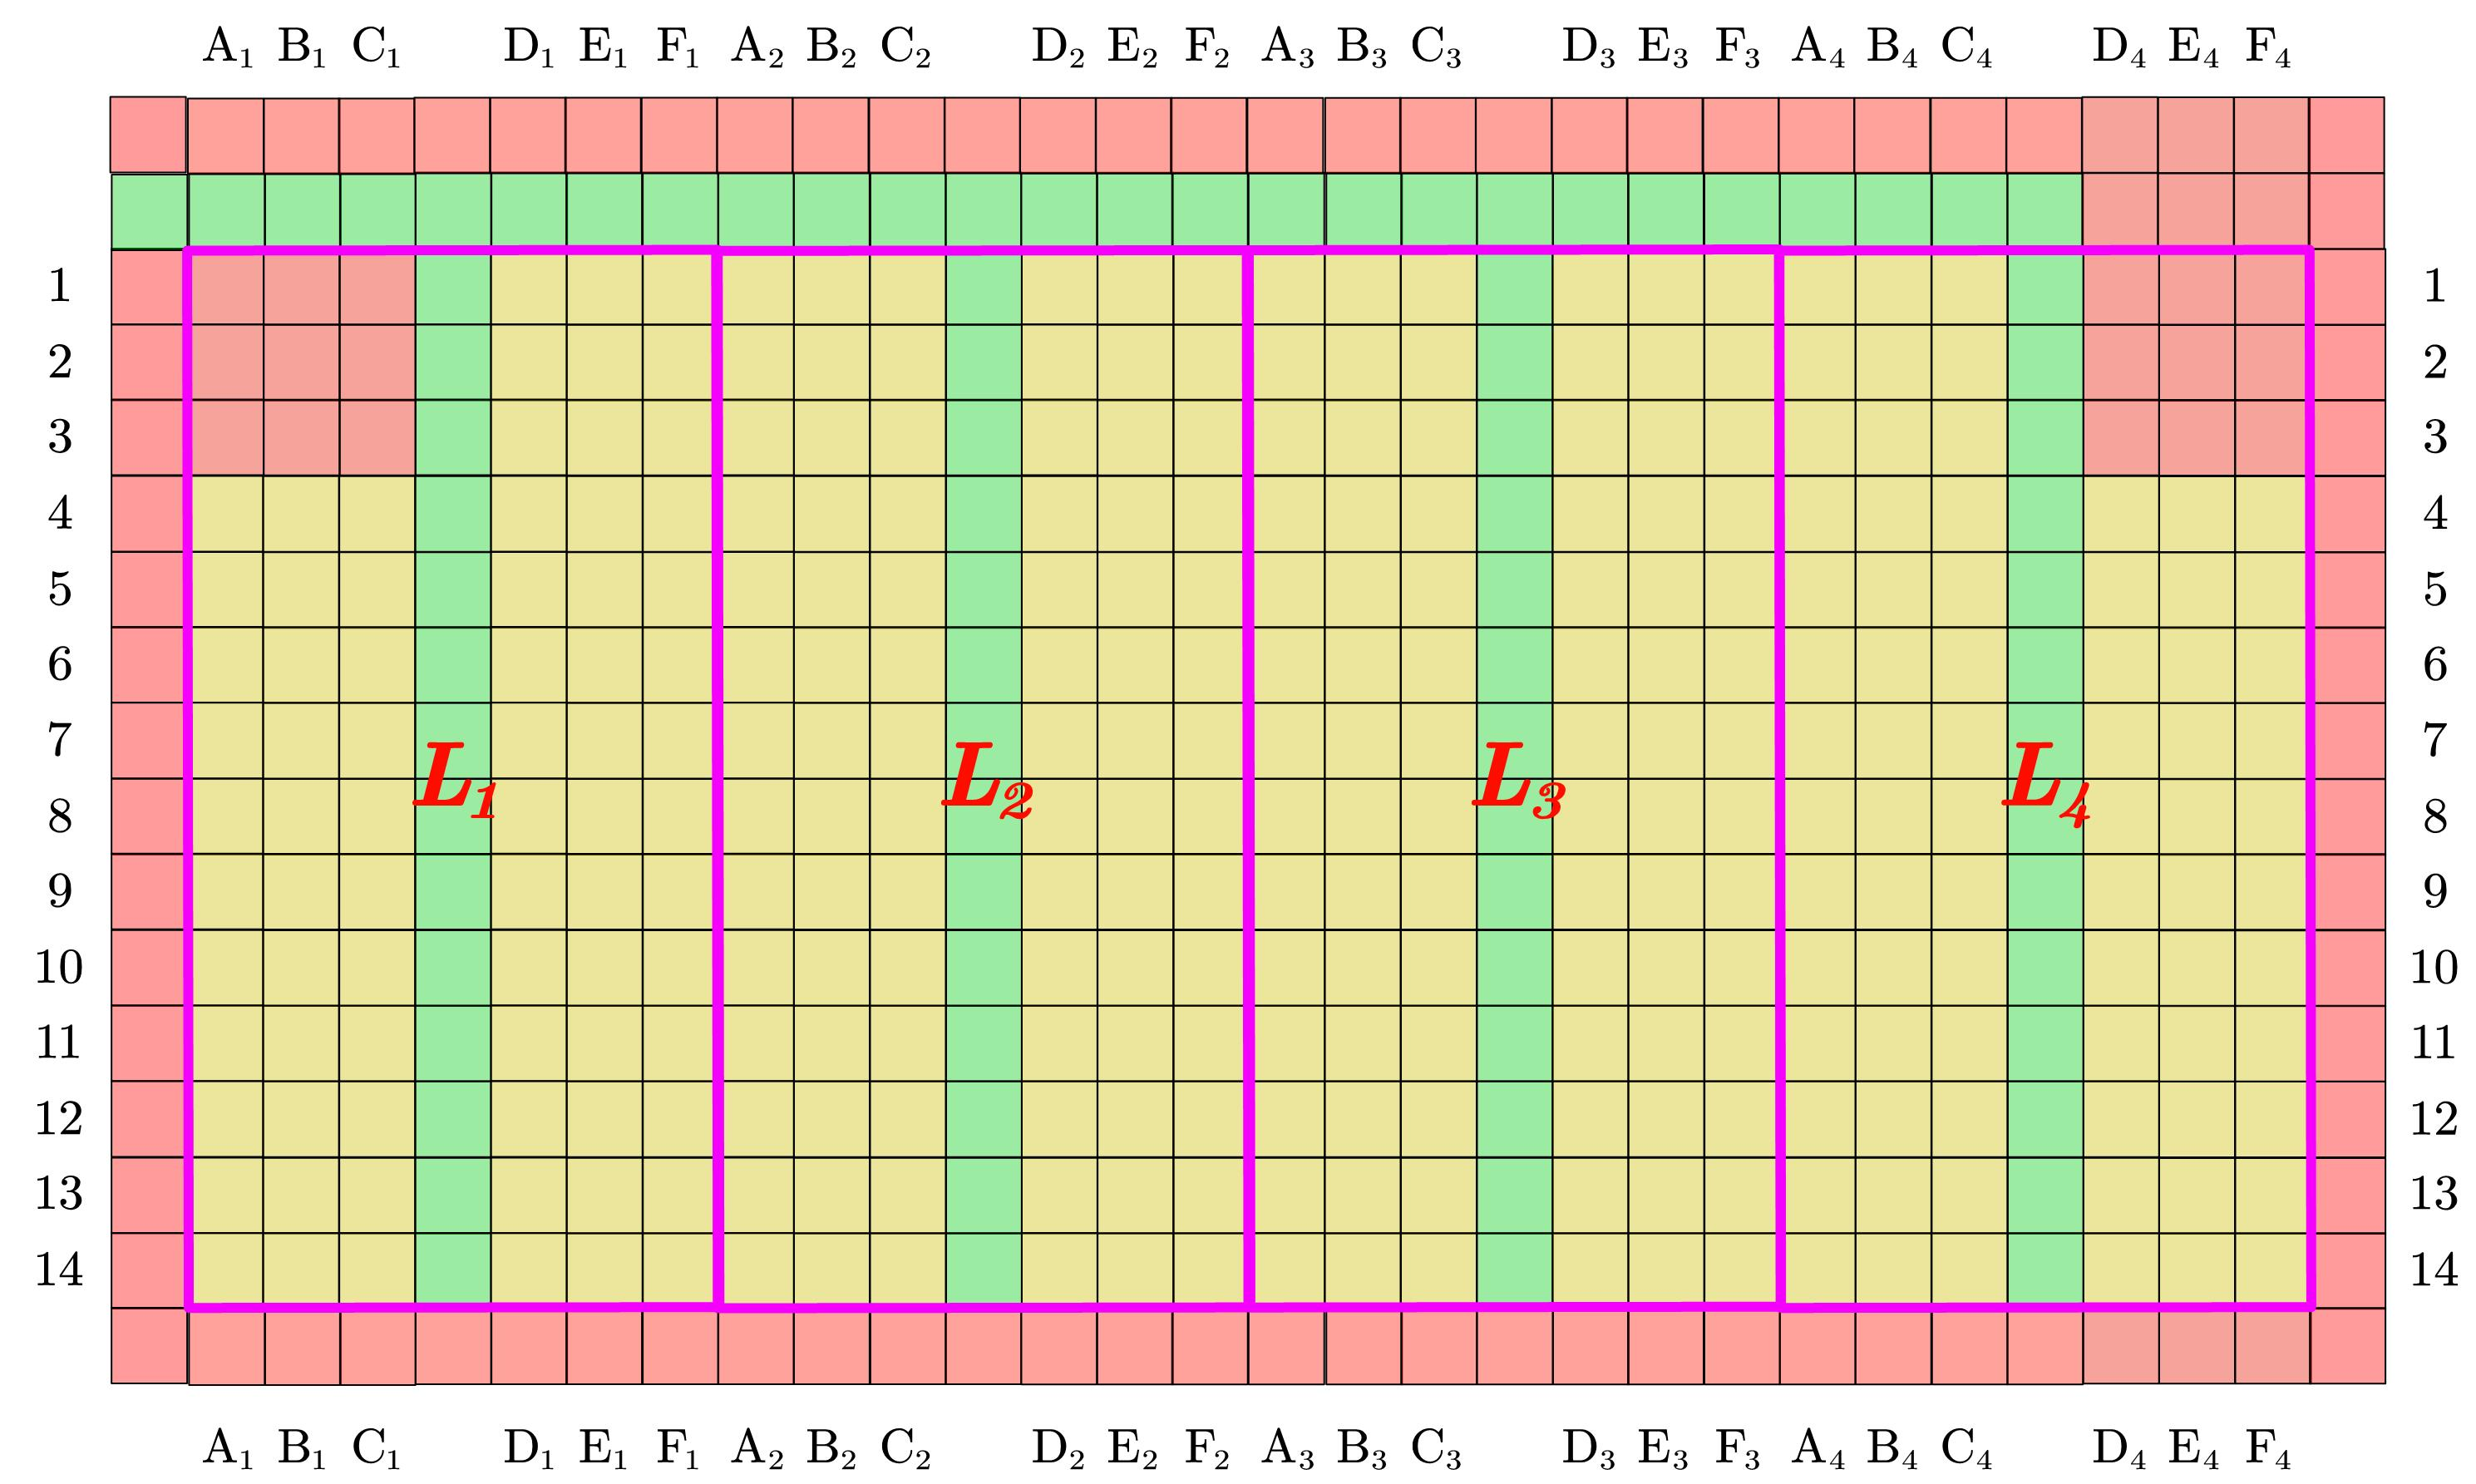
\includegraphics[width=12cm]{flyingwings.jpg}

		\small \textit{Fig. Flying Wings}
	\end{center}

	\subsection{}


	\section{Strengths and Weaknesses}
	\subsection*{Strengths}
	\begin{itemize}
		\itembf{}
	\end{itemize}
	\subsection*{Weaknesses}
	\begin{itemize}
		\itembf{}
	\end{itemize}




	\newpage
	\section{Letter to the Airline Executive}
	\noindent Dear airline executive:

	We are the \defword{IMMC Mathematical Modeling Group}.


	\newpage
	%\setcounter{page}{\wholepages}
	\renewcommand\refname{References}
	\addcontentsline{toc}{section}{References}
	\tolerance=500
	\begin{thebibliography}{100}
	\bibitem{passenger} \textit{Lorentzian-geometry-based analysis of airplane boarding policies,highlights “slow passengers first” as better},
	Sveinung Erland, Jevgenijs Kaupužs, Vidar Frette, Rami Pugatch and  Eitan Bachmat
	\bibitem{steffen} hello
	\end{thebibliography}

	\newpage
	\thispagestyle{empty}
	\renewcommand\refname{Appendix}
	\Huge \textbf{Appendix}
	\\[0.8cm]
	\large \textbf{Back to Front}
	\begin{center}
		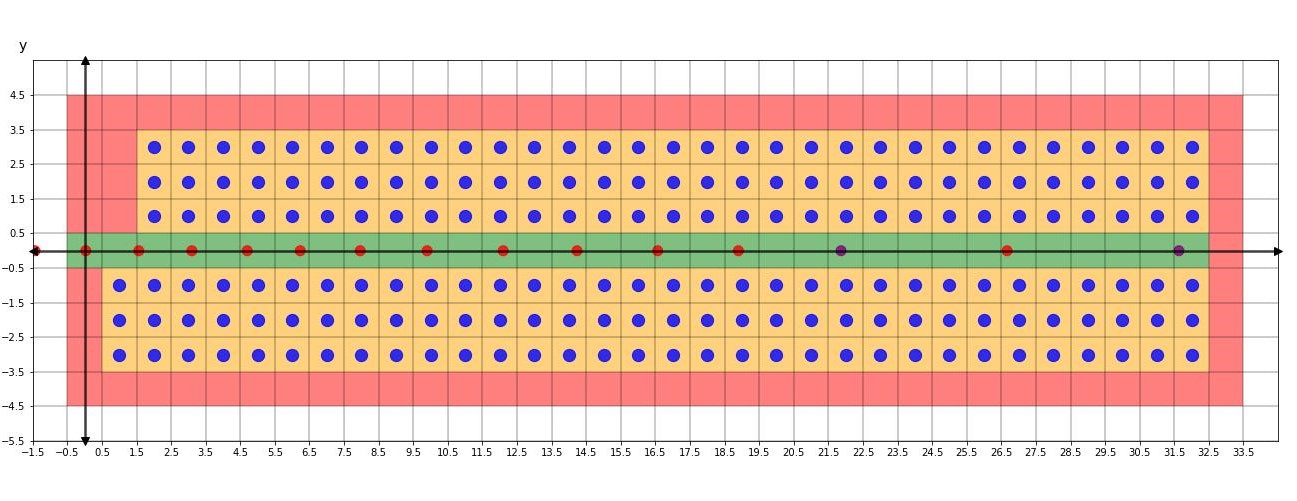
\includegraphics[width=14cm]{backtofront1.jpg}\\
		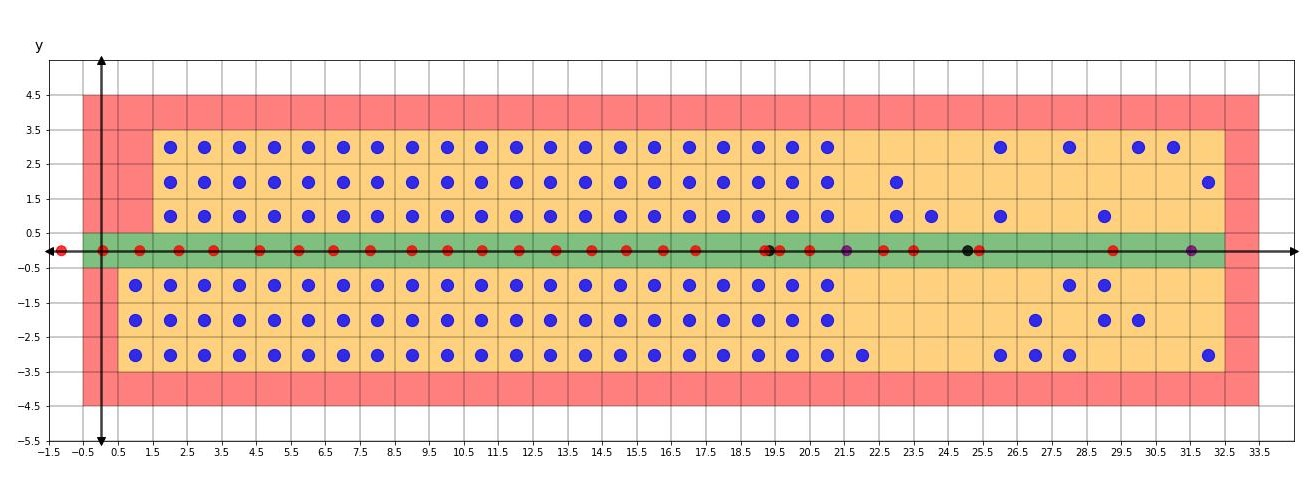
\includegraphics[width=14cm]{backtofront2.jpg}\\
		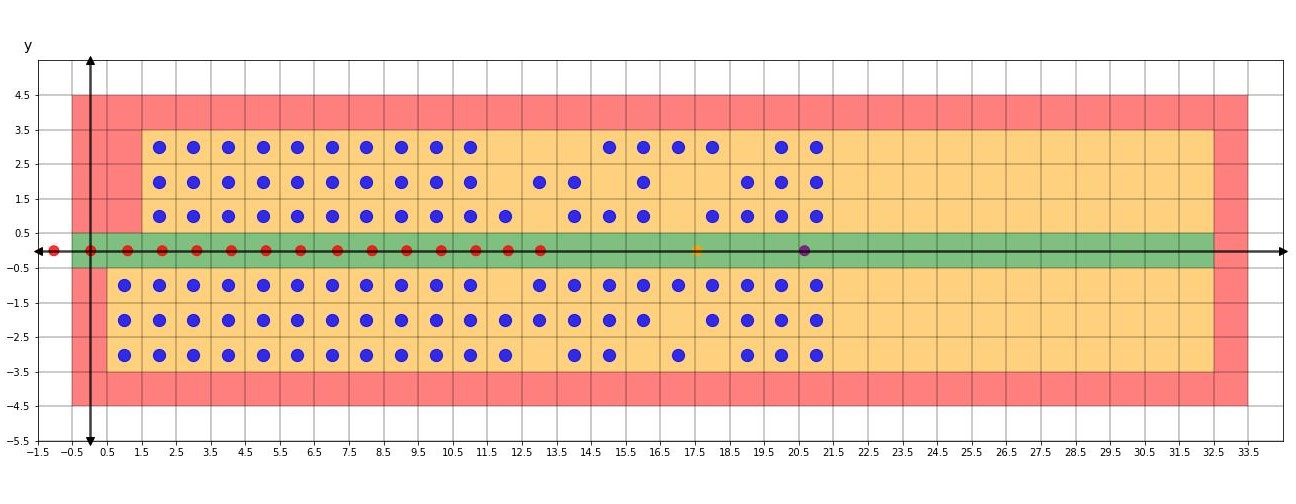
\includegraphics[width=14cm]{backtofront3.jpg}\\
		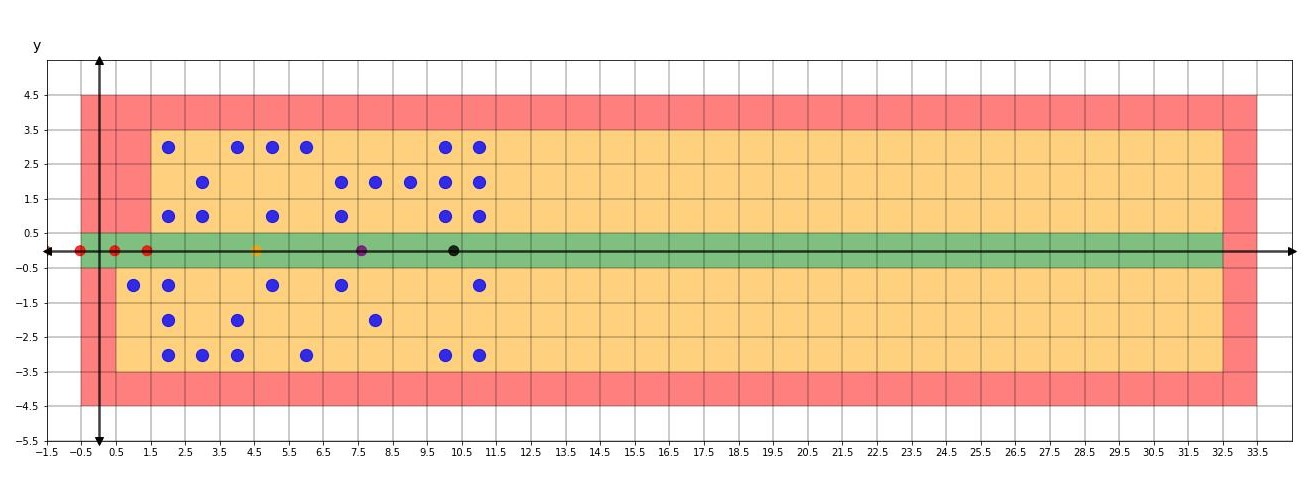
\includegraphics[width=14cm]{backtofront4.jpg}\\
	\end{center}
	\tolerance=500
\end{document}
